% Change to 'masters' to produces the masters thesis preliminary pages
\documentclass[oneside,phd,etd]{UoBclass}

\usepackage{import}

% preamble contains title page, signature page, acknowledgement and abstract texts
\usepackage{_preamble}

% Packages used
\usepackage[utf8]{inputenc} % Remove warning on ascii conversion
\usepackage[T1]{fontenc} % Remove warning on ascii conversion
\usepackage[refsection=part,citestyle=apa,style=authoryear,natbib=true,backend=biber]{biblatex}
\usepackage{hyperref}
\usepackage{fancyhdr}
\usepackage{acronym}

% Make chapter numbers into string words 1 -> ONE
\usepackage{fmtcount}
\makeatletter
\renewcommand*{\lstlistlistingname}{List of Code Snippets}
\renewcommand{\@makechapterhead}[1]{\vspace *{40\p@ }{\parindent \z@ 
\raggedright \normalfont \ifnum \c@secnumdepth >\m@ne \Huge \bfseries 
\@chapapp \space \Numberstring{chapter} \vskip 10\p@ \fi #1\par \nobreak \vskip 30\p@ }}
\makeatother

\pagestyle{fancy}
\fancyhf{}
\fancyhead[R]{\leftmark}
\renewcommand{\chaptermark}[1]{\markboth{#1}{}}
\cfoot{\thepage}

\addbibresource{_bib.bib}

\begin{document}

\hypersetup{breaklinks=true}

 % Start page counting in roman numerals
 \frontmatter

 % This command makes the formal preliminary pages.
 % You can comment it out during the drafting process if you want to save paper.
 \makepreliminarypages

 \doublespace
 % Make the table of contents.
 \tableofcontents
 \thispagestyle{plain}
 
  % Make the list of figures
 \mylistoffigures
 \thispagestyle{plain}

 % Make the list of tables
 \mylistoftables
 \thispagestyle{plain}
 
 % Make the list of listings
 \lstlistoflistings
 \thispagestyle{plain}
 
 % This page is OPTIONAL. To remove, comment out and \dedicationpage in _thesis.tex
 %\dedicationpage
 \clearemptydoublepage
 
 \chapter*{List of Acronyms}
 \begin{acronym}[]
     \acro{AWS}{Amazon Web Services}
     \acro{ASVS}{Application Security Verification Standard}
     \acro{CI}{Continuous Integration}
     \acro{CD}{Continuous Development}
     \acro{C5}{Cloud Computing Compliance Controls Catalogue}
     \acro{DSL}{Domain Specific Language}
     \acro{DVWA}{Damn vulnerable web app}
     \acro{FST}{Functional Security Testing}
     \acro{MBST}{Model-based security testing}
     \acro{MBVT}{Model-based vulnerability testing}
     \acro{OWASP}{Open Web Application Security Project}
     \acro{PoC}{Proof of Concept}
     \acro{RAII}{Resource allocation is initialization}
     \acro{SecurityRAT}{Security Requirements Automation Tool}
     \acro{SecurityCAT}{Security Compliance Automation Tool}
     \acro{SEP}{Security Engineering Process}
     \acro{SLA}{Service Level Agreement}
     \acro{SUT}{System under Test}
     \acro{TaRA}{Threat and Risk Analysis}
     \acro{ZAP}{ZED Attack Proxy}
\end{acronym}
\thispagestyle{plain}

 % Start regular page counting at page 1
 \mainmatter

% OK. Everything is set up. Type your thesis here.
\addchapheadtotoc
\chapter{Introduction}
This chapter gives a brief introduction on the topic of automated security testing and aimed at goal for the proof of concept implementation of the Security Compliance Automation Tool. Additionally, it describes the structure of this thesis to provide the reader with a guide.

\section{Introduction}
News about data breaches and leaks is ubiquitous. Even though many of the exploited vulnerabilities are known security issues, most products and services do not see the threat. The high cost of security experts further supports this problem. Many companies are not able to focus their financial assets on security-related topics.
Pipelines for source code analysis and functional test automation are part of all major software companies. However, automated security and system compliance tests are not. For many corporate environments, software projects have to comply with a set of defined requirements before releasing them to production. Those requirements are tested manually by a security expert.

This thesis proposes a tool that enriches available tooling for requirement management, like SecurityRAT, with a set of automation services. The Security Compliance Automation Tool (SecurityCAT) provides interfaces for simple extendability and consists of reusable components. Evaluation for requirements of different standards like ASVS \citep{asvs4.0} or C5 \citep{bsiC5} can be delegated after configuration.


\section{Task and Goal of this Thesis}
This thesis serves as a baseline test for the feasibility of adding a Compliance Automation Tool (CAT) to the cloud security evaluation process at a company. Based on requirements defined at the company, a proof of concept system has been implemented, which provides capabilities to test infrastructure level, as well as application-level requirements in an automated manner.

The single central source of truth is a tool called SecurityRAT. It defines projects - called artifacts - for different use cases like the onboarding of an Azure project. Requirements suitable for Azure are then automatically selected from the company internal catalog of requirements. Tests for specific requirements can then be triggered by this tool. The according results are added to the tested requirements upon evaluation completion. 

A final evaluation will enable the teams - that use SecurityRAT - to assess if using SecurityCAT will improve and optimize their pipeline. In addition to that, the open-source CAT provides a fully documented architecture and an interface definition for customizations and extendability.


\section{Structure of the Thesis}
This thesis is written in a way that separates the theoretical basics from the practical implementation of the Compliance Automation Tool (CAT). By doing this, readers can skip over the fundamentals if they are already aware of testing approaches and security automation essentials. 

The first Chapter, "Fundamentals", introduces basic concepts and keywords, as well as current standard approaches to security testing, both manual and automated. It describes the relation between traditional software testing and security testing and references related work.

After listing different approaches, Chapter 3 evaluates the suitability of those approaches for the scope of the task. 
Chapter 4 introduces the current testing approach and explains what SecurityRAT is and how it is used.

The actual implementation of the proof of concept is covered in Chapter 5. It displays the thoughts behind the architecture, implementation details, and provides an outlook for the extendability of the taken approach.

The final Chapters summarize the usability and workability of the Proof of Concept (PoC) and evaluate whether it is useful in the provided context.
\definecolor{gainsboro}{rgb}{0.90, 0.90, 0.90}

\addchapheadtotoc
\chapter{Fundamentals}
The following chapter introduces basic terms and concepts that play an essential part in understanding the complexity of software security testing. It presents conventional approaches and briefly explains the approach taken in this thesis.

\section{Testing Approaches}
\subsection{Model Based Testing}
In the software development process, model-based testing describes the automated generation of test cases based on a formal model of the system under test (SUT). It checks the correctness of a system by performing experiments in a systematic and controlled way. \citep{torxAMBT2003}

Model-based testing is led by an oracle that runs assertions for test generation and execution.
The test oracle collects the results from the tests and creates reports out of it. \citep{sypolt2018}

\newpage 

\begin{figure}[ht!]
\begin{center}
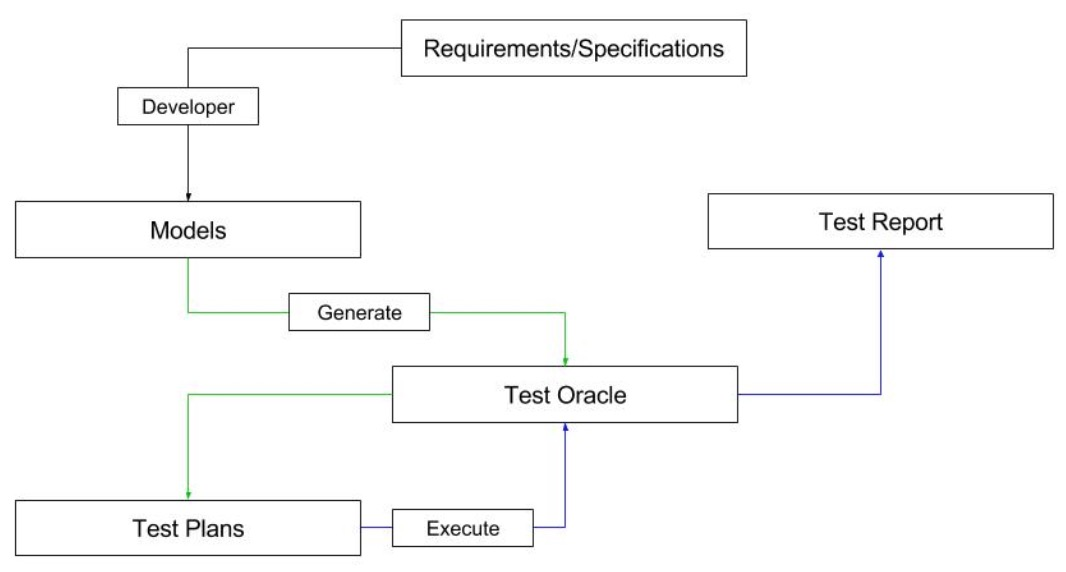
\includegraphics[height=8cm]{modelbasedtesting_sypolt.jpg}
\end{center}
\caption[Model Based Testing Schema - Role of the testing oracle]{Model Based Testing Schema - Role of the testing oracle. Graph from \citep{sypolt2018}}
%Source:
\label{fig_devsecops}
\end{figure}

The general rule with model-based testing is that the success of a given model is based on the quality of the model. \citep{mbsvt2007}
Functional models typically describe the behavior, while architectural models define the configuration of a system. \citep{mbst2012}
An example of the later will be covered in \ref{infrastructure_testing} using Azure Policies.

Model-based security testing (MBST), in addition to functional testing, consists of approaches such as model-based fuzzing, risk and threat oriented testing, and the usage of security patterns. MBST has a more complex scope since functional hazards, such as accidental mistakes on implementation, are simpler to find than persistent security threats. \citep{mbst2012}

Model-based vulnerability testing (MBVT) is an even more specific field of application for the model-based paradigm. \citep{mbsvt2007}
Vulnerabilities are mostly not related to the functional requirements of the application. Rather they are sensitive to implementation details, which requires thought-through planning. \citep{mbvtWA2013}


\subsection{Planning Based Testing}
\label{planningBased}
Testing based on planning is comparable to the model-based testing approach. The automatic generation of test cases also needs some model of the to be tested system. 
One of the differences is that planners (planning based tools) also create an attack plan and then transform the plan into suitable test cases \citep{wotawa2014}.

The concept of planners is common for intelligent agents and autonomous systems. Transitions, and action sequences, are generated that transition the agent from the initial state into the given goal state.
The objective of planning based security testing is to ensure that applications reliably handle well-known attack patterns by modeling the attack as a sequence of known actions that are carried out in a specific order.

Instead of finding new vulnerabilities, handling known attacks is the focus of a planning-based approach.
In \citep{wotawa2014} the authors introduce an algorithm called PLAN4SEC which makes use of an ordinary planner that is provided with a problem and domain description based on the Damn Vulnerable Web App (DVWA).

Below is an example of a generated testing plan of a given domain and problem description from \citep{wotawa2014}.

\begin{lstlisting}[ backgroundcolor = \color{gainsboro}, 
                    xleftmargin = 2cm, 
                    framexleftmargin = 1em, 
                    language=R,
                    caption={Planning Based Testing DSL Example},
                    captionpos=b]
0: START X URL LO
1: SENDREQ X LO SE SI
2: RECREQ X SI
3: PARSE X M USERNAME PASSWORD TYPE 
4: CHOOSERXSS X TYPE
5: ATTACKRXSS X XSSI M UN PW
6: PARSERESPXSS X SCRIPT RESP
7: PARSERESPXSSCHECK X SCRIPT RESP 
8: FINISH X
\end{lstlisting}

This generated plan is expressed in a domain specific language (DSL) which is parsed by JavaFF \citep{javaffColes}. The according Java functions for each instruction are then executed in order.

\subsection{Test Automation}
Even considering the existence of Model- and Planning based testing approaches, the most prominent approaches to testing are still manual \citep{secTestingSurvey2016}.
Replacing this repetitive manual execution by non-complex scripts and automation is the chosen approach in this paper.

Creating and establishing one of the more complex approaches requires specialized knowledge in both the domain and the abstraction process. The more common approach in software projects, see \ref{current_testing_etas}, is to either contract another department or company with the testing. Manually writing unit, integration, and regression tests for the most critical and feasible elements, as well as a Continuous Integration (CI) / Continuous Development (CD) pipeline for static code analysis, is also prominent \citep{secTestingSurvey2016}.

In the scope of vulnerability testing, for example, approaches like fuzzing, dir busting, and SQL injection can be used to find the so-called "low hanging fruit" and harden the project against very basic attacks \citep{autoPentestOverview2018}.

\newpage

\section{Security Testing}
\subsection{Compliance and Governance}
Compliance and Governance ensure the alignment of a given system with requirements, controls, and industry standards.
Even though they are both meant to protect an organization form the same threats and risks, they need to be looked at separately.

Both terms and concepts are crucial for understanding the role they play in the security testing process, as well as the importance of the Azure microservice implemented in this thesis.

\subsubsection{Compliance}
According to the Cambridge Dictionary, the term "compliance" describes the conformity of a system to a set of given rules and requirements \citep{compliance2020}.
This means that a system must meet those requirements in order to conform to the regulations and rules of the organization. 

In the context of software systems, requirements can be both organizational and technical. Organizational measures consider the conceptual requirements of a system, like defining and designing an access role concept. In contrast, technical measures define less abstract and more testable requirements like the state and format of logging in our applications. 

Compliance is only one of the conceptual entities combined in the process of Governance.

\subsubsection{Governance}
\citep{bannerman2009} describes Governance as "a multi-dimensional concept, encompassing elements of organizational stewardship, accountability, risk management, compliance, control, propriety, functional oversight, resource allocation, and capability. It tends to be defined from one of two perspectives: functionally, in terms of what Governance does (e.g., assigning and administering decision rights, responsibilities, and accountabilities) or; structurally, in terms of what it looks like (a framework of interrelated boards, councils, and committees)."

In the domain of software development, Governance can be described as a mechanism to ensure that defined engineering and business needs are met. Software development governance defines processes for "the assignment and maintenance of software development capability decision rights, governance responsibilities and accountabilities; software development capability planning, monitoring and review processes; issue escalation procedures, and stakeholder consultation" \citep{bannerman2009}.


\subsection{Static Application Security Testing (SAST)}
The "Static Source Code Analysis", as the name suggests, is performed without executing the program. It is a fundamental approach to review the formal correctness, data-flow, and even credential leaks.
Static code analysis is generally implemented as one of the first gates of continuous integration pipelines.

Depending on the focus of the analysis, there are different state-of-the-art providers for static code analysis like for example credential checking on Open-Source platforms like GitHub using GitGuardian \citep{gitGuardian2020}.

When focusing on security testing with static analysis, problems that can be identified with high confidence have to be targeted. Those include, for example, SQL Injections and Buffer Overflows.
The OWASP-project provides a list of tooling that can \citep{owaspStaticTools2020} be used as part of a continuous integration pipeline. 
Once a vulnerability is found, the build fails and provides detailed reporting to the developers who have to fix the issues before future builds succeed.

However, this approach has many drawbacks. It has a high rate of false positives, which can significantly increase the time needed for manual testing and reviewing.
In addition to that, most security vulnerabilities are difficult to find automatically. Access control issues or the insecure use of cryptography are only a few examples. Even misconfigurations cannot be identified without a model-based approach, as discussed before.

A more recent approach, Semmle QL, uses variant analysis to find problems in code based on a similar, known vulnerability. Code is treated as data and fed into the CodeQL engine together with custom queries that perform data analysis and track down known vulnerabilities \citep{semmle2020}. 

A straightforward query for finding all the comments that contain a \enquote{TODO} looks like the following.

\vskip 1cm

\begin{lstlisting}[ backgroundcolor = \color{gainsboro}, 
                    xleftmargin = 2cm, 
                    framexleftmargin = 1em, 
                    language=SQL,
                    caption={Semmle QL TODO Query},
                    captionpos=b]
import python

from Comment c
where c.getText().regexpMatch("(?si).*\\bTODO\\b.*")
select c
\end{lstlisting}


Much more complex queries for cases such as buffer overflows, critical recursion, or DOM XSS attack vectors are available. 
This approach enables more in-depth static analyses that can eliminate common known vulnerabilities.


\subsection{Functional security testing (FST)}
In the context of software development, functional testing can cover different scopes. When done in an isolated environment rather than an operational context, it is called "Unit Testing". When tested together with other applications of the system, it is called "Integration Testing" \citep{warren2011}.

Functional security testing, on the other hand, is focused on ensuring that applications do not act in ways they are not meant to, regardless of the scoping. The critical element of this approach is "Negative Testing," which tests explicitly for misbehavior, for example, on the corrupted or wrong input. Given the vast amount of attack vectors, this is a broad and open-ended task.

According to \citep{warren2011}, this approach can give some level of assurance in terms of the avoidance and resistance to attacks.


\subsection{Security Vulnerability testing (Penetration Testing)}
\label{securityVulnerabilityTesting}
According to \citep{mcgraw2006}, "Penetration Testing is a comprehensive method to test the complete, integrated, operational, and trusted computing base that consists of hardware, software, and people."

It is an analysis of the system for potential vulnerabilities such as hardware and software flaws and faulty system configuration. Even operational weaknesses and employee manipulation, with so-called Social Engineering, can be in scope for the test \citep{mohanty2020}.

Given the strong fan-out of attack vectors, penetration testing requires highly skilled candidates with a particular skillset focusing on the to be tested infrastructure and application \citep{bacuidoYuanChuJones2011}.

Penetration testing is different from functional security testing in a way that FST checks the correct behavior of the system's security controls. Penetration testing, in contrast, determines the difficulty for someone to penetrate an organization's security controls \citep{autoPentestOverview2018}.

In a study conducted by the German Federal Office for Information Security \citep{bsiStudy2020}, the five phases of the Penetration Testing process are defined as follows.

\begin{figure}[ht!]
\begin{center}
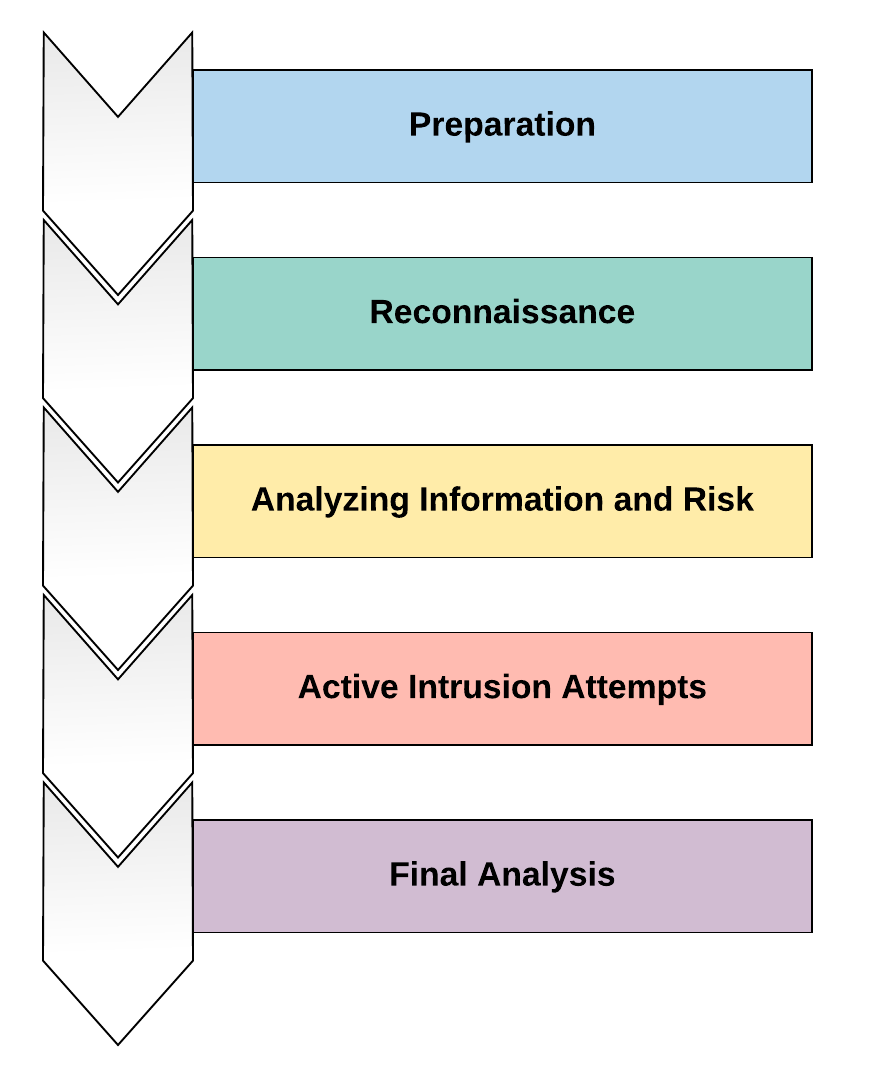
\includegraphics[height=10cm]{Pentesting_Process.png}
\end{center}
\caption[Penetration testing process flow - according to \citep{bsiStudy2020}]{Penetration testing process flow - according to \citep{bsiStudy2020}}
%Source:
\end{figure}

\newpage

\subsubsection{Phase 1: Preparation}
In the first phase, requirements and objectives, as well as procedures of the test, have to be defined with the client. The project has to be scoped and should be written down in the contract to avoid any legal infringements.

\subsubsection{Phase 2: Reconnaissance}
Reconnaissance is a strategic observation. In the second phase, a complete and detailed overview of the system, including possible attack vectors, is gathered and documented.

\subsubsection{Phase 3: Analyzing information and risks}
Phase 3 can act as a funnel to further filter down possible targets. The process of Threat and Risk Analysis (TaRA), as it is called at the security consulting team at the ETAS GmbH, includes defined goals for the test, potential risks to the system, and an estimate of the time required for system evaluation. 

\subsubsection{Phase 4: Active intrusion attempts}
Given the outline and analysis from previous phases, this phase covers the attack on the defined system to the in the analysis defined extend.

On systems with high availability or integrity requirements, potential adverse effects have to be considered in advance. For those systems, patches to prevent full system failures might be installed before testing. 

\subsubsection{Phase 5: Final analysis}
The last phase defines the requirements for report generation. The final report should "contain an evaluation of the vulnerabilities located in the form of potential risks and recommendations for eliminating the vulnerabilities and risks". It also has to disclose the done tests and found vulnerabilities. \citep{bsiStudy2020}


This manual process is time and resource-intensive while parts of it, especially reporting, are highly repetitive and display a high potential of automatability \citep{passi2018}.


\newpage

\section{Automated Testing}
\subsection{On the need for Automated Testing}
With the alarming amount of data breaches in recent years \citep{dataBreaches2019}, the need for security testing is more profound than ever before.
Many projects and even companies do not have access to security professionals due to the low number of available specialists and the time and cost intensity of such tests \citep{autoPentestOverview2018}.
Automated security testing, e.g., testing phases integrated into a continuous integration pipeline, could help to roll out underlying security testing mechanisms on a large scale.
Re-runnable and, especially, reproducible security testing as part of the release process that provides detailed automated reports can drastically increase the basic level of security of an application without the need for security specialists. \citep{vijayan2019}.

One of the biggest challenges for automated testing, however, is the absence of a strict model of the system. Without a formally given configuration of the system, deciding what is wrong or right relies on human decisions. There is no strict right or wrong in some cases \citep{mbst2012}.
Completely removing manual testing, as of now, is not feasible since automated processes do not have the intuition and lateral thinking of a human tester \citep{portswigger2020}.


\subsection{Automated Resource Compliance Testing with Policies}
\label{infrastructure_testing}
Since cloud resources, most of the time, are declared through a process called Infrastructure as Code, we have a specific model and reproducible configuration to base the testing on. 
These so-called templates define e.g., the type of the resource, the version, and properties like the amount of storage and CPU. Every attribute of the resource is defined through this configuration \citep{awsIac2017}. If values are not defined, they are assigned a set default value.

The structure and elements of such a configuration depending on the platform or cloud provider. For Microsoft Azure, the resource management system enables the use of e.g., built-in validation, policies as code, and CI/CD integration \citep{azureResourceTemp2020}.

A very simple example of such a resource manager template can look like this:

\begin{lstlisting}[ backgroundcolor = \color{gainsboro}, 
                    xleftmargin = 2cm, 
                    framexleftmargin = 1em, 
                    language=JSON,
                    caption={Microsoft Azure Resource Manager VM Template Snippet},
                    captionpos=b]
{
  "$schema": "https://schema.management.azure.com/schemas
              /2015-01-01/deploymentTemplate.json#",
  "contentVersion": "1.0.0.0",
  "resources": [
    {
            "type": "Microsoft.Compute/virtualMachines",
            "apiVersion": "2019-03-01",
            "name": "simpleLinuxVM",
            "location": "[resourceGroup().location]",
            "properties": {
                "hardwareProfile": {
                    "vmSize": "Standard_B2s"
                },
                ...
            }
        },
        ...
  ]
}
\end{lstlisting}

The above-displayed configuration is far from complete. However, it displays enough information to communicate the basic structure of such a template file. The templates create a new "B2s" computing instance and assign it to the location of the resource group. Properties like whether file encryption is active or if backups are enabled can, therefore, be checked using Azure Policies. Amazon Web Services has a comparable system called AWS CloudFormation templates \citep{awsCloudFormation2010}. The capabilities are similar, the format, however, is a little bit different.
A comparable configuration, like the one shown for Microsoft Azure, for AWS looks like this:

\begin{lstlisting}[ backgroundcolor = \color{gainsboro}, 
                    xleftmargin = 2cm, 
                    framexleftmargin = 1em, 
                    language=JSON,
                    caption={AWS EC2 Instance Template Snippet},
                    captionpos=b]
{
    "AWSTemplateFormatVersion": "2017-01-09",
    "Description": "Launch an EC2 Instance with 
                    defined properties",
    "Resources": {
        "SecureInstance": {
            "Type": "AWS::EC2::Instance",
            "Properties": {
                "ImageId": "ami-31814f58",
                "InstanceType": "t2.nano",
                "KeyName": "key-pair",
                ...
            }
        },
        ...
    }
}
\end{lstlisting}

With the given configuration, we launch a new t2.nano EC2 computing instance with the given properties set.

Using the Infrastructure as Code approach brings many more advantages than trivial compliance testability of resources. Reproducibility, management, monitoring, and optimization are streamlined through this code-centric approach \citep{awsIac2017}.

\begin{figure}[ht!]
\begin{center}
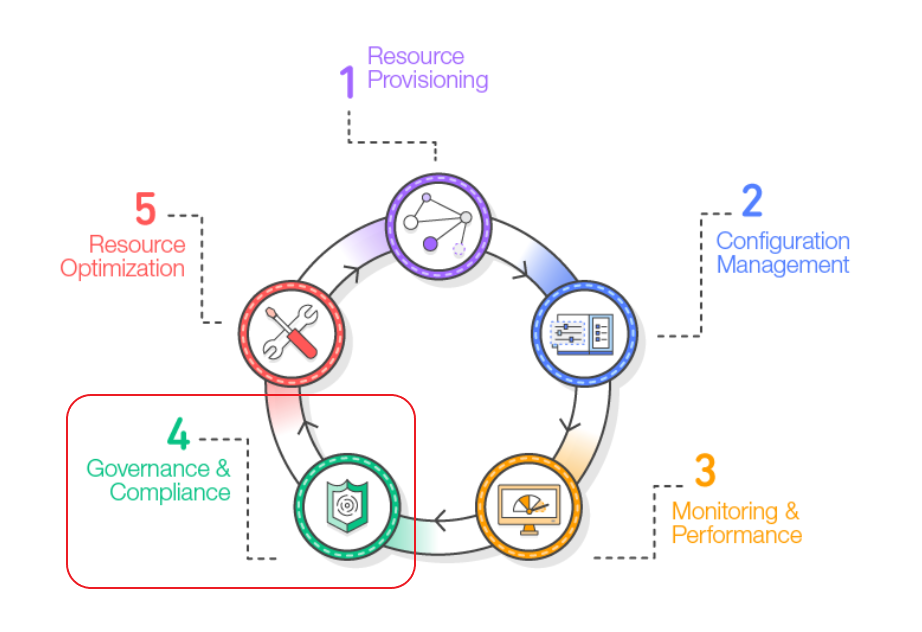
\includegraphics[height=8cm]{annotated_aws_iac_lifecycle.png}
\end{center}
\caption[Infrastructure resource lifecylce according to AWS]{Infrastructure resource lifecylce according to AWS. Drawing from \citep{awsIac2017}}
%Source: https://d0.awsstatic.com/whitepapers/DevOps/infrastructure-as-code.pdf
\label{fig_devsecops}
\end{figure}

Policy compliance testing for cloud resources is one of the processes for which a concept of automation was implemented in this thesis. Advance to \ref{automated_infrastructure_testing} to read about the concrete implementation further.

\newpage

\subsection{DevSecOps}
The concept behind DevSecOps integrates automated security testing into the continuous quality assurance of continuous development, integration, and deployment. 
It combines Development, Security, and Operations to improve the speed, turnover time, and overall quality of products.
Manual security and compliance testing slows down release processes and therefore needs to be augmented with automated testing and integrated into the continuous software deployment lifecycle.

\begin{figure}[ht!]
\begin{center}
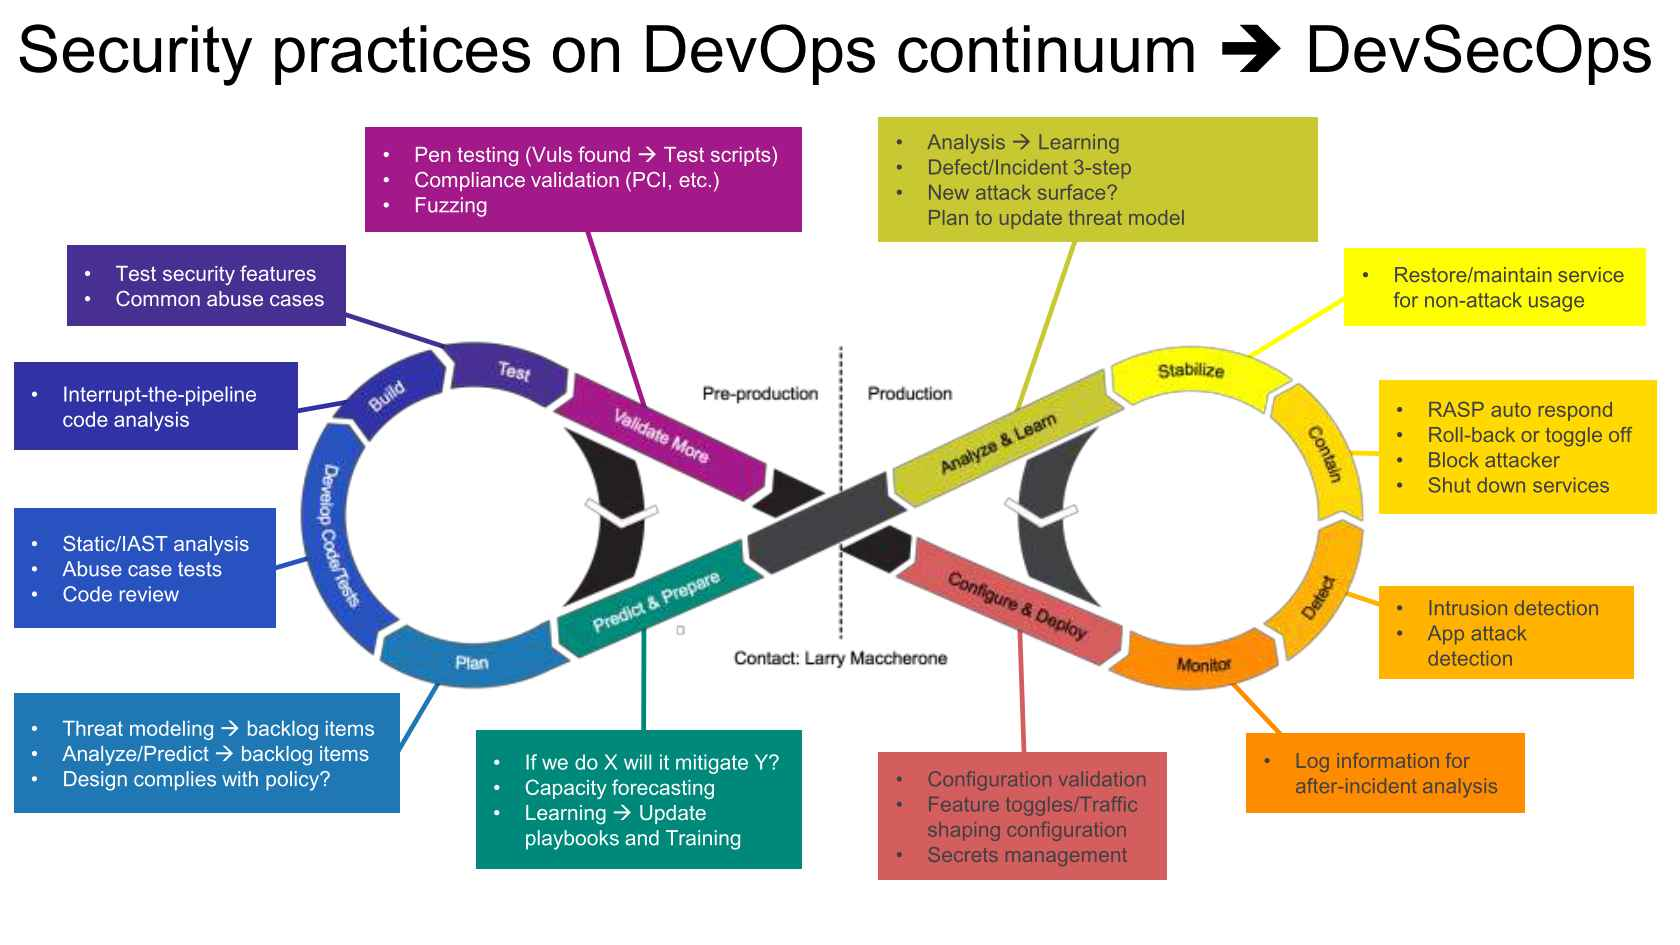
\includegraphics[height=8cm]{devsecops.jpg}
\end{center}
\caption[DevSecOps - Security practices on DevOps continuum]{DevSecOps - Security practices on DevOps continuum. Graph from \citep{alicloud2018}}
%Source:
\label{fig_devsecops}
\end{figure}

The schematic drawing of DevSecOps displays and explains the significant elements of the life cycle.
Security is implemented in the overall process, and breaches in security or compliance lead to interrupted releases.
In the operations phase, intrusions are detected, countermeasures taken, and attacks analyzed, which enables reporting that can be leveraged to improve the quality and security of the product in the development phase.
When observing the DevSecOps cycle in more detail, the discrepancy of fighting insecure software with a lot of organizational rituals instead of simplifying the security analysis becomes present.

\subsection{Automated Penetration Testing}
\label{autoPentTesting}
As stated in \ref{securityVulnerabilityTesting}, penetration testing itself is an approach that requires highly specialized testers. Automating this process could benefit smaller companies that lack the resources to hire specialized teams to test their projects.

Penetration tests should be performed whenever new software is installed, user policies are modified, security patches applied, or new infrastructure is added to the system \citep{autoPentestOverview2018}.
Manually testing all the components this often is a luxury only few can afford. Automating this process and making it part of the CI/CD pipeline would drastically increase the level of security of a project \citep{stefinko2016}.

Popular tooling for automated penetration testing are OWASP's ZAP \citep{zapProxy}, Burpsuite \citep{burpSuite}, Metasploit \citep{metasploit}, and, for cloud systems like AWS, Pacu \citep{pacu}. All of those tools, however, only automate parts of the attacks like, for example, executing known vulnerabilites.  

The system implemented in this thesis makes use of the ZED Attack Proxy (ZAP). In \ref{zapTesting}, ZAP is used to test for, so called, "Low hanging fruit". Basic misconfigurations and exposed data that can be found by a general scan and attacks based on findings.

\newpage

\begin{figure}[ht!]
\begin{center}
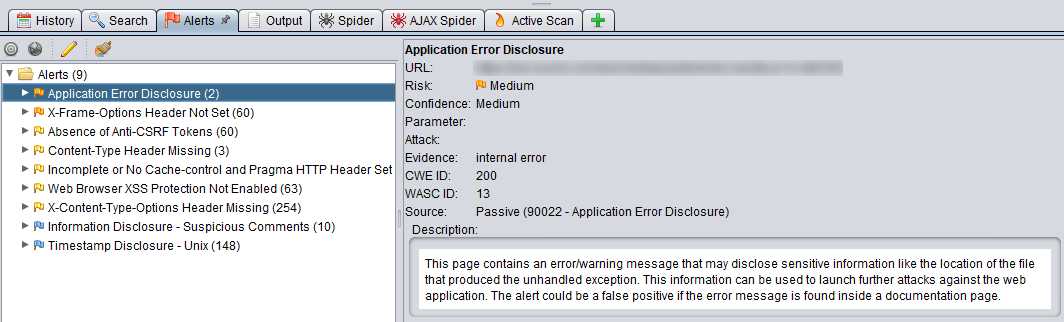
\includegraphics[width=17cm]{zap_example_report.png}
\end{center}
\caption[ZAP report structure example]{ZAP report structure example}
%Source:
\end{figure}

After spidering, scanning and attacking a web application, ZAP provides a report that summarizes different alerts with their severity, the confidence that this problem is present and a possible solution. This information can be used to define whether certain requirements are fulfilled or not.


\subsection{Drawbacks of automated testing}
\label{drawbackAutomated}
At first, automating security tests sounds feasible. Considering the sheer complexity of applications and their possibly infinite attack surface, however, it becomes clear that using automation faces many challenges \citep{stefinko2016}.
A general problem with automated tests is the possibility and, often, a high amount of false positives. 

Especially automated penetration tests lack the experience and intellect of a professional tester that uses pivoting to attack the network and other machines once one machine is compromised \citep{stefinko2016}.
Most popular test automation tools can only leverage vulnerabilities that have already been reported \citep{autoPentestOverview2018}. One of the most significant risks of relying on automated testing is the false sense of security and invincibility that can result from withstanding a defined range of security testing. Real attacks are more complex and can leverage unexpected attack vectors \citep{stefinko2016}.


\section{Related Work}
\label{relatedWork}
The need for novel approaches and automation for security testing becomes present when observing the wide variety of papers published on according ideas and frameworks.
The idea to use similar approaches to security testing based on software functional testing is prominent in model-based testing described in, for example, \citep{torxAMBT2003}. It introduces an abstract framework for automated model-based testing, which can be adapted for security-related topics.
Other approaches, like planning-based testing, as described in \ref{planningBased}, introduce planners and a specific language to describe attack vectors. The implementation of PLAN4SEC in \citep{wotawa2014} provides both examples of a possible framework and the effectiveness of such an approach.

When looking at more concrete implementations for cloud \citep{cloudSec2017} and mobile application \citep{androidTesting2012} security testing, awareness for the enormous value of automating those repetitive processes with a rerunnable continuous deployment emerges. More complex topics, such as automated penetration testing, however, need a lot more research and, most likely, the usage of specialized AI systems in order to provide better and more reliable results than efforts recorded in \citep{autoPentestOverview2018} and \citep{automatedPentesting2011}.


\section{Evaluating and selecting a suitable approach}
The wide range of possible approaches opens up the discussion about which is the \enquote{right one}. Model- and planning-based approaches may provide more reliable results in the long run. However, since the goal of this thesis is to implement and evaluate tooling to test both infrastructures with an underlying defined configuration, and application which comes with the drawbacks explained in \ref{relatedWork}, a more general approach to test automation with \enquote{custom scripts} is taken.

\ref{infrastructure_testing} introduces the underlying concept of infrastructure testing. Compared to security vulnerability testing (\ref{securityVulnerabilityTesting}), a more model-driven approach is already present and provided by cloud providers. The scope of interaction is restricted, which reduces complexity and enables high confidence evaluations to be tested resources.
Considering those advantages, a custom interactor for the Microsoft Azure Policy service was implemented.

Keeping the abstraction on a high level and leveraging the application universality of the ZAP Proxy allows the application level microservice to run a baseline of general tests against any web application. This, however, increases the number of false negatives and reduces the amount of found application-specific vulnerabilities.
For the first proof of concept implementation, this is feasible and can be improved upon functional validation of the setup.

An additional microservice for more specific tests of HTTP responses - like checking for required headers in HTTPS requests - is also added to the system. As described in \ref{customTestingScript}, it holds a mapping between some internal requirements and an execution flow on how to test the given requirement according to application.

All decisions have been taken with consideration on the requirements maintained in SecurityRAT and adjusted towards a consistent architecture and usage described in \ref{extendability}.
\addchapheadtotoc
\chapter{An approach to automated testing using a Requirement Automation Tool (RAT)}

This chapter describes the tools and standards used in the current manual testing approach and illustrates the importance of SecurityRAT.

\section{Current testing workflow}
\label{current_testing_etas}

\subsection{Open Web Application Security Project (OWASP)}
The Open Web Application Security Project, short OWASP \citep{owasp2020}, is a non-profit organization that aims to improve web application security by providing freely available educational material. The material includes different tooling, on-demand videos, forums, and extensive documentation. 
The OWASP project is mostly known through the open-source projects, created and maintained by the community.
One of their most famous projects is the OWASP Top 10 \citep{owaspTopTen2020}, which lists the most common vulnerabilities for web applications. The Application Security Verification Standard \citep{owaspAsvs2020} is another of OWASP's popular flagship projects. 


\subsection{Application Security Verification Standard (ASVS)}
\label{asvsStandard}
The Application Security Verification Standard, short ASVS, is a community-driven project that aims to provide a baseline of security controls for web application testing.
It was developed with two main uses in mind. 
As a metric, it supports developers to estimate the "degree of trust" \citep{asvs4.0} that can be placed in their applications.
As a guide, it provides a base for application security requirements in contracts. It tells developers what security controls need to be built into the application to comply with the given requirements.

ASVS can be used to establish a level of confidence in the security of Web applications \citep{asvs4.0}. This is achieved by defining three levels, which are categorized as follows.

\begin{itemize}
    \item Level 1 is for low assurance levels and is completely penetration testable. 
    
    \item Level 2 is for applications that contain sensitive data, which requires protection and is the recommended level for most apps.
    
    \item Level 3 is for the most critical applications - applications that perform high-value transactions, contain sensitive medical data, or any application that requires the highest level of trust.
\end{itemize}
\citep{asvs4.0}

\subsection{Cloud Computing Compliance Controls Catalogue (C5)}
The C5, published by the Federal Office of Information Security, provides a set of criteria to assess the information security of cloud services \citep{bsiC5}.
Since there is no defacto standard, only several context-specific standards, C5 aids customers to get an overview at a higher level of security. 

It is divided into 17 sections that define requirements for different domains, including standard information security entities like "Cryptography and key management", and also more organizational domains like "Personnel", which assures that employees are aware of their responsibilities and the confidentiality of the assets they handle. 

C5 itself builds on top of national and international standards such as ISO/IEC 27001, the Cloud Controls Matrix, the BSI IT-Grundschutz, and German standards such as BSI SaaS Sicherheitsprofile \citep{bsiC5}.

\subsection{OWASP SecurityRAT}
The OWASP Security Requirement Automation Tool, short SecurityRAT, is an application designed to streamline the management of security requirements throughout the development process.
It comes with an initial set of requirements stated in the ASVS. Users, however, are encouraged to create their own set of requirements since risk profiles differ significantly between companies.
SecurityRAT emphasizes automation over merely listing requirements. Properties of an application in development are specified, then used to filter down the set of requirements only to get the ones that have to be fulfilled. 

The set of requirements, for example, contains elements specific to Microsoft Azure Implementation. Each "Implementation Type" has it is own given set of requirements.

\newpage

The requirements can be annotated about whether they have to be implemented or not. In addition to that, the reasoning or result can be documented in SecurityRAT.

\begin{figure}[ht!]
\begin{center}
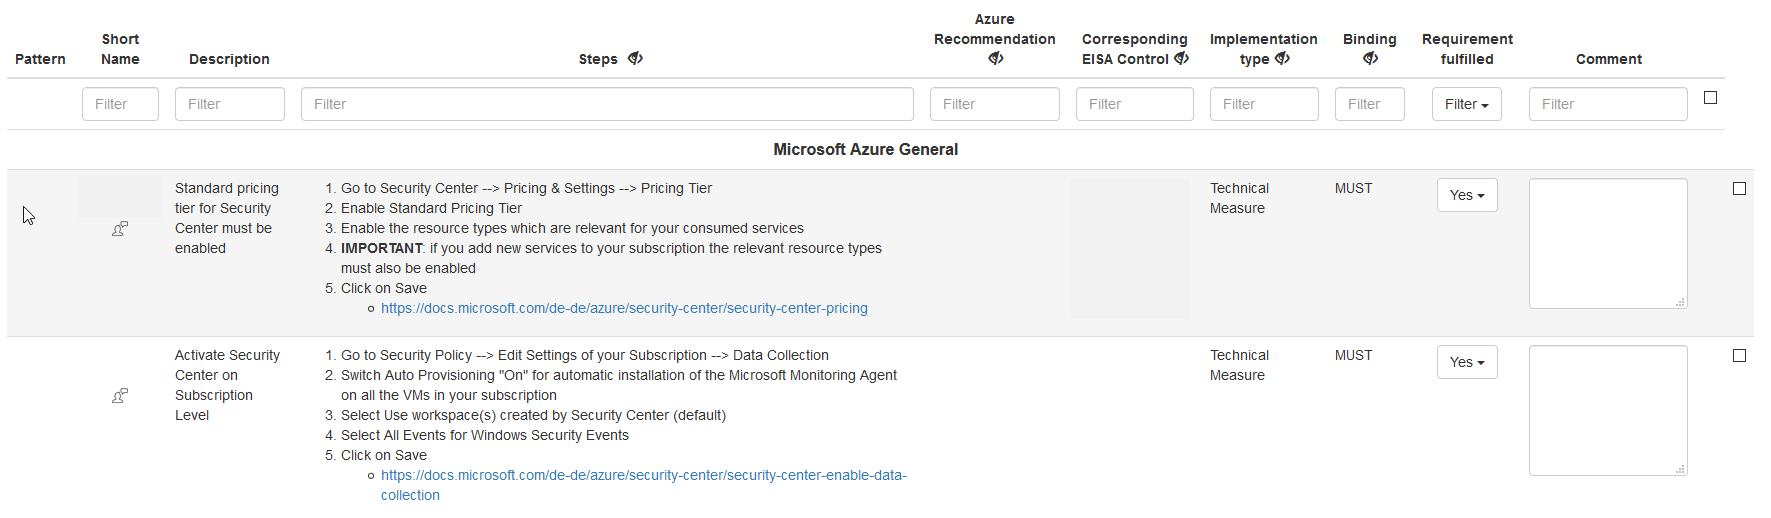
\includegraphics[height=5cm]{secrat_screen.png}
\end{center}
\caption[Screenshot of SecurityRat]{Screenshot of SecurityRAT Microsoft "Azure Implementation Guide" requirements.}
%Source:
\label{fig_devsecops}
\end{figure}

The focus on automation becomes present through the integration of JIRA into the tool. JIRA tickets can automatically be created, tracked, and documented with SecurityRAT.

\begin{figure}[ht!]
\begin{center}
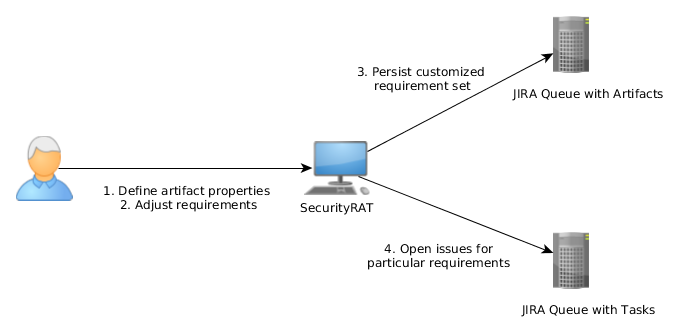
\includegraphics[height=8cm]{security_rat.png}
\end{center}
\caption[SecurityRat Schema]{Schematic drawing of SecurityRAT process flow. Graph from \citep{secrat2020}}
%Source: https://securityrat.github.io/
\label{fig_devsecops}
\end{figure}

\vskip 1cm

The process flow of SecurityRAT can be described as follows:

\begin{itemize}\itemsep0pt \parskip0pt \parsep0pt
    \item Property specification of the software project, called artifact 
    \item Common security requirements are listed as a subset of the given requirements database
    \item Decide which requirements are needed and how they are handled
    \item Create automated JIRA tickets for state tracking of open issues
\end{itemize}

SecurityRAT provides additional automation for project excel sheet export, training slides creation, and with SecurityCAT, automated testing of trivial technical measures.


\section{Adding a Compliance Automation Tool (CAT)}
\label{secCat}
SecurityRAT is a tool designed for the management and handling of security requirements. Even though it has some convenience automation features like the above mentioned excel sheet export, it does not provide automated testing of system compliance to security requirements.

SecurityRAT exposes a REST API that allows to plug in other systems. SecurityCAT is a proof of concept implementation of such a system focused on compliance and security evaluations. It consists of a gateway and several use-case specific microservices that can be used to test the according to requirements automatically. According to the needs, those microservices can be set up or not. The detailed explanation of the structure and architecture of SecurityCAT is described in \ref{architecture}.

\newpage

\begin{figure}[ht!]
\begin{center}
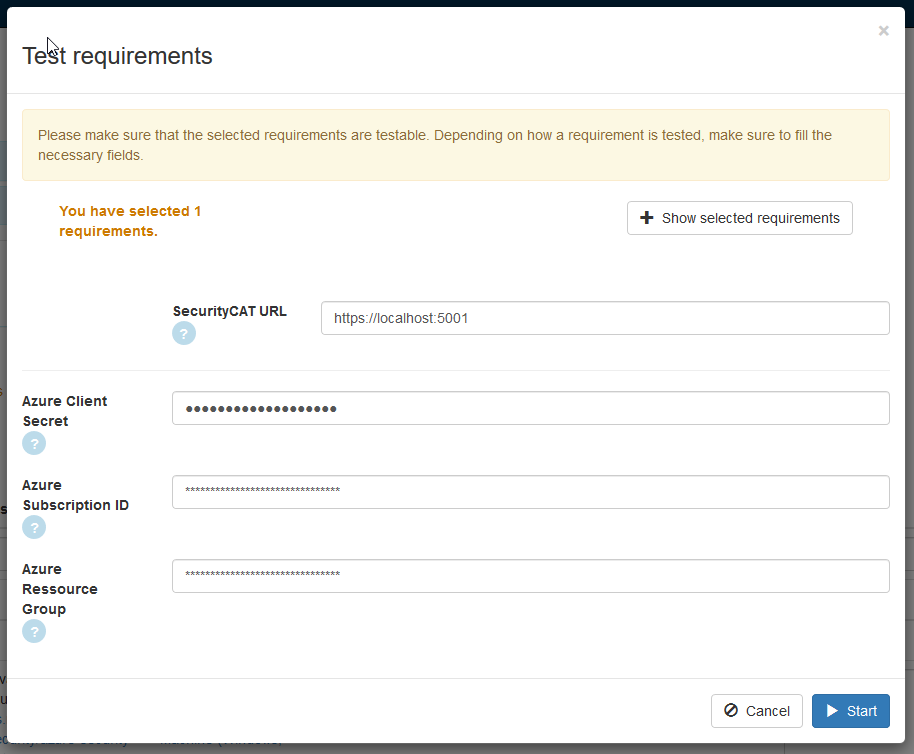
\includegraphics[height=12cm]{secrat_test_requirements_widget.png}
\end{center}
\caption[SecurityRat test execution widget for SecurityCAT]{SecurityRat test execution widget for SecurityCAT}
%Source:
\label{fig_devsecops}
\end{figure}

By jointly incorporating the execution of automated testing into SecurityRAT, the whole process of evaluating a project is meant to be streamlined and parallelized. The figure above shows the test execution widget within SecurityRAT that is used to trigger, and therefore delegate, the execution, and evaluation of the selected requirements. 
To better identify requirements that can be tested in an automated manner, they will get a unique tag that identifies them and therefore make them easy to filter.
\addchapheadtotoc
\chapter{Security CAT - Proof of Concept Implementation}

This chapter introduces the Proof of Concept setup and architecture of the Security Compliance Automation Tool. It gives an overview of general components and the implemented microservices. 

\section{Architecture}
\label{architecture}
Considering the nature of the testing and evaluation system described in \ref{secCat}, a microservice architecture with loose coupling of the core components, is required. Simple extendability and delegation from SecurityRAT are the focus points in the design.
The architecture incorporates already validated efforts done in \citep{secCat2020}. Parts of the architecture have been adjusted to support lengthy running evaluations and increase the level of abstraction.

The below schematic drawing visualizes the entities and interconnections of SecurityCAT.

\newpage

\begin{figure}[ht!]
\begin{center}
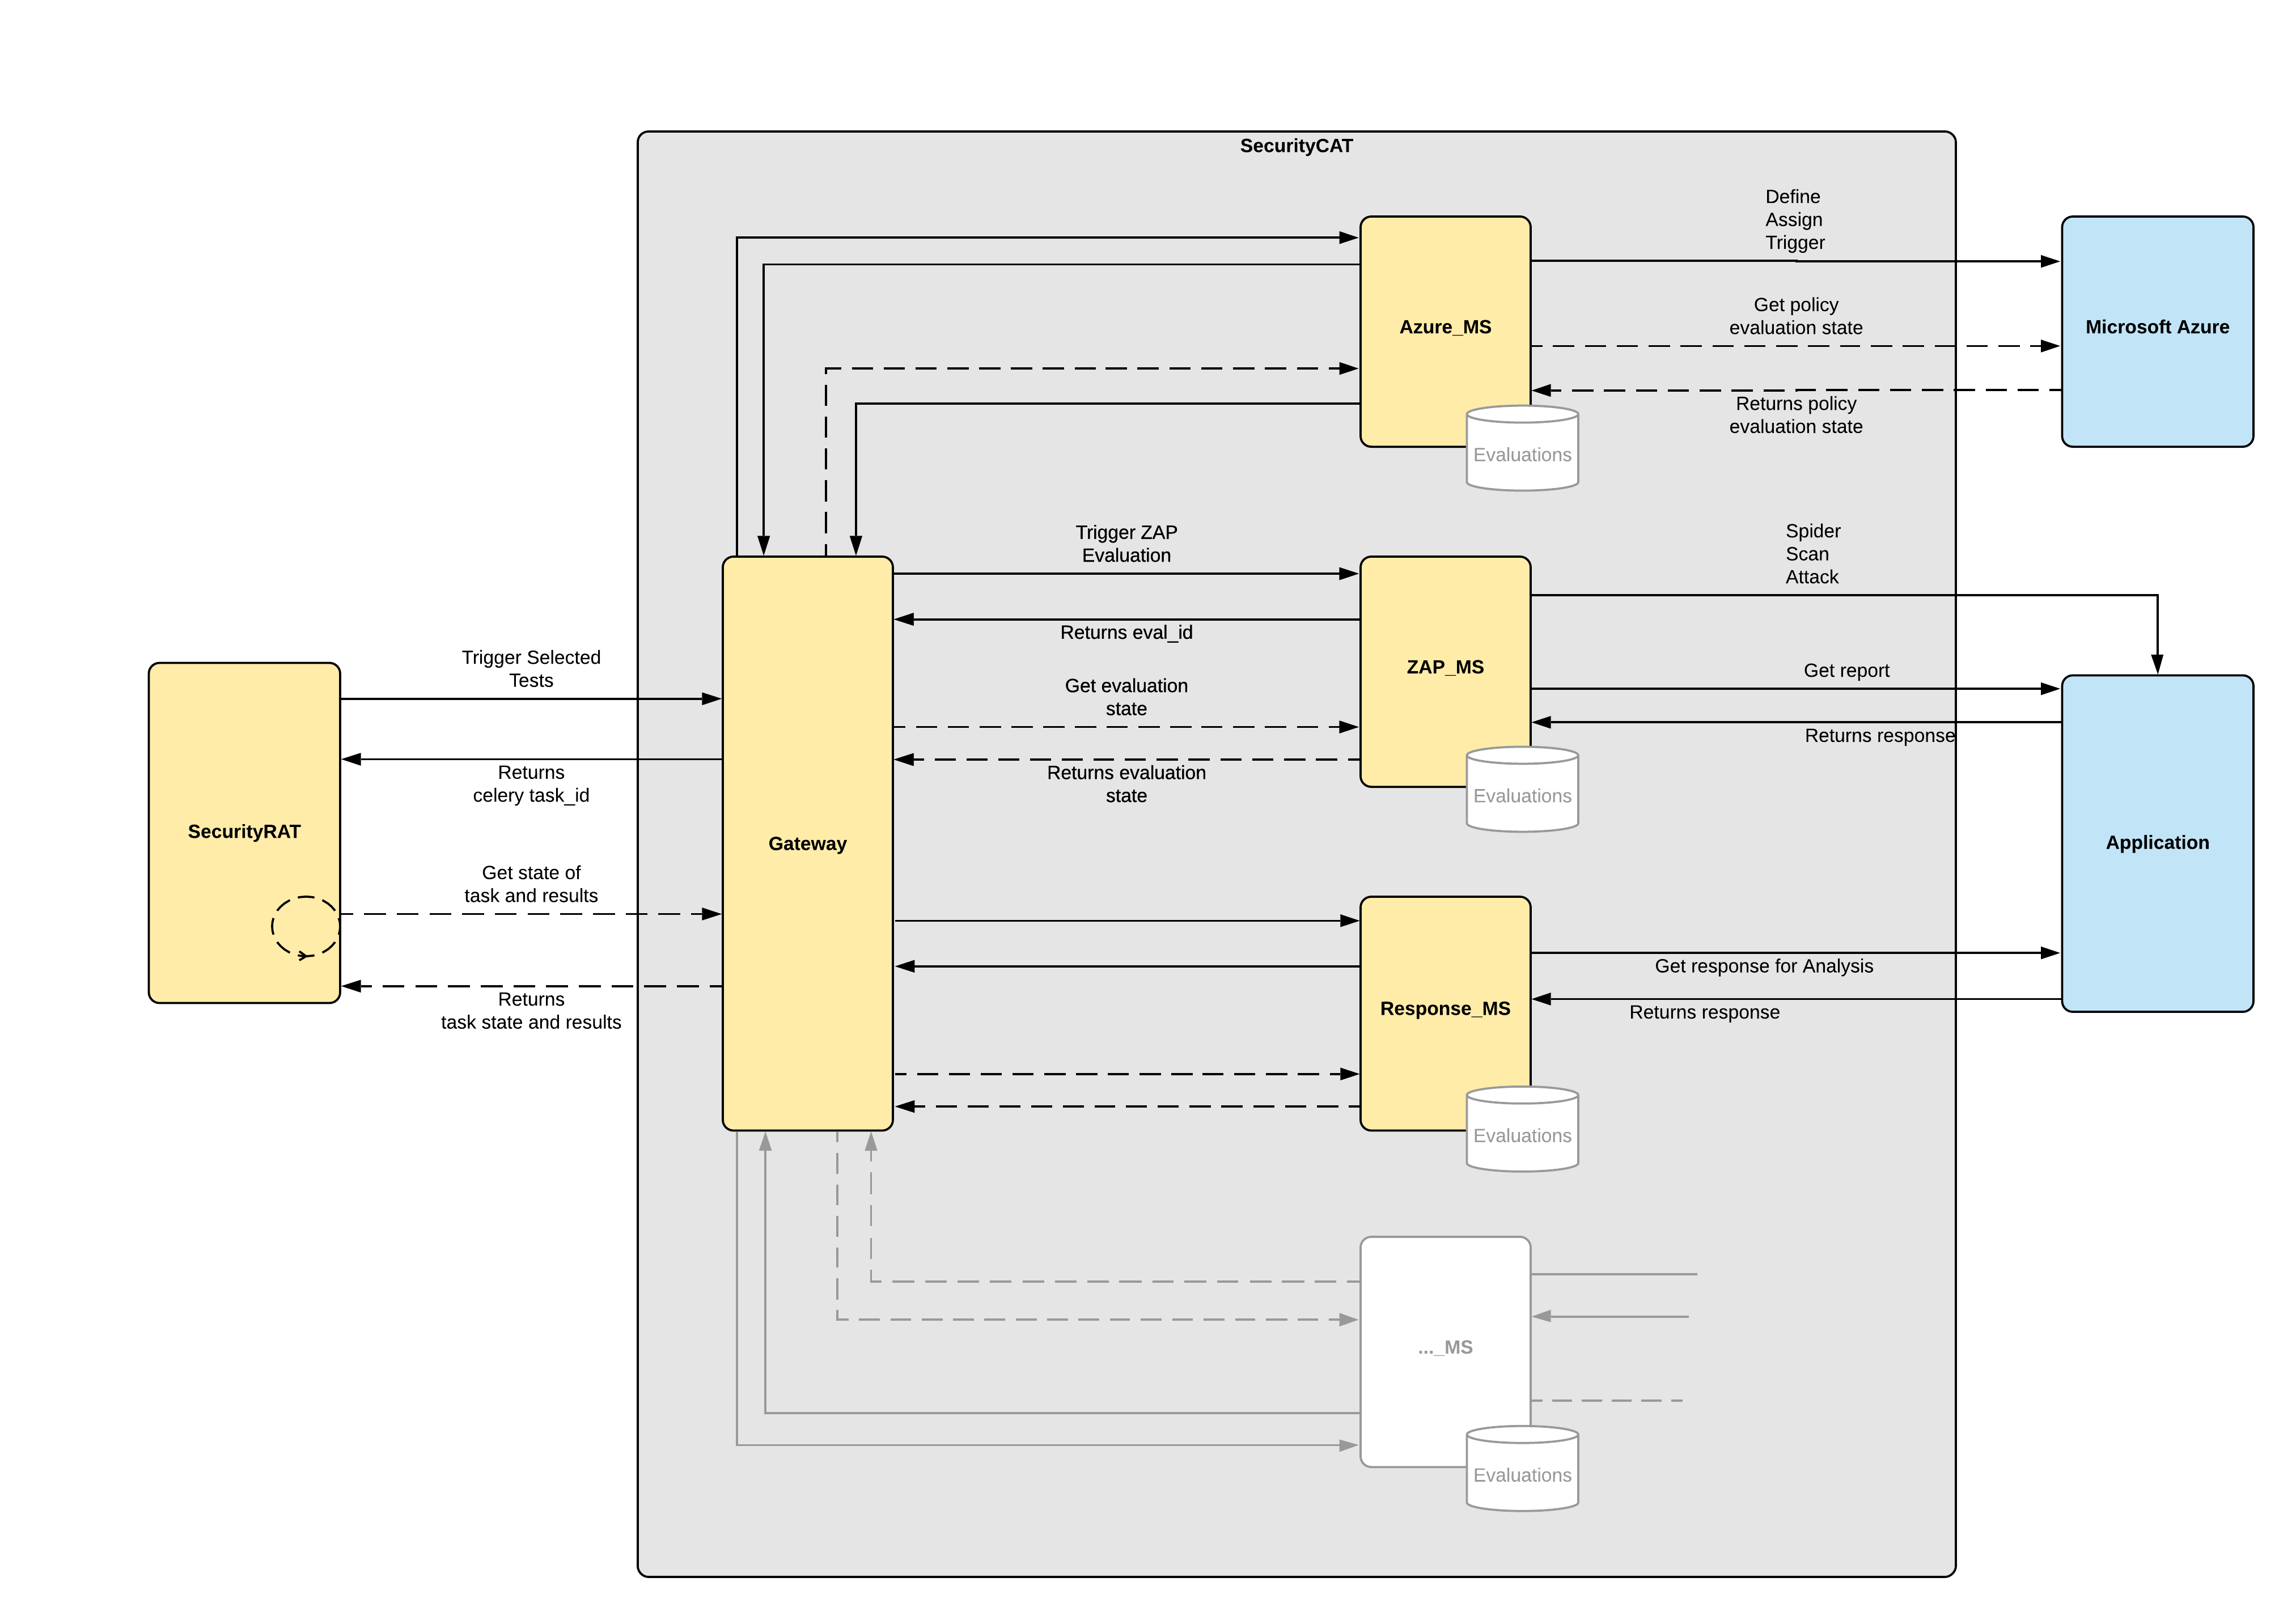
\includegraphics[width=17cm]{SecurityCAT_Architecture.png}
\end{center}
\caption[SecurityCAT architecture]{SecurityCAT architecture}
%Source:
\end{figure}

SecurityRAT serves as a single source of truth for the management of the given project. Only information persisted in SecurityRAT is recognized as acceptable, and any information gathering starts there.

Selecting and testing requirements trigger the process of delegating them to the gateway of SecurityCAT. The gateway further delegates the requirements to the microservices depending on the to be tested properties. SecurityCAT creates a celery task for each test evaluation and returns the according to celery \boldsymbol{task\textunderscore id} to SecurityRAT. This \boldsymbol{task\textunderscore id} is then used to check the progression state and result of the evaluation regularly with a given interval.

Each microservice is passed only the information necessary for the evaluation. Upon triggering the test evaluation, a microservice returns a \boldsymbol{eval\textunderscore id} to the gateway. This \boldsymbol{eval\textunderscore id} is used to check the state of evaluation once SecurityRAT checks in at the gateway for the state of test evaluation.
Each microservice has its additional elements described in their according sections of this thesis. They are not displayed in the architectural overview. Resources that are accessed and used are not part of SecurityCAT and are defined by the properties defined in the SecurityRAT test creation step.

New microservices can be added by following the format given in \ref{extendability}. The system flow allows long-running and time-consuming evaluations. Especially the policy and compliance evaluation of Microsoft Azure can take several minutes depending on the size of the infrastructure.


\section{Automated Infrastructure Testing}
\label{automated_infrastructure_testing}

\subsection{Microsoft Azure Policies}
Not every internal requirement is easily testable with a given Azure policy. Organizational requirements, as stated before, as well as more complex technical requirements like protection against application-level security threats, can not be tested this way.

Upon triggering of the test execution, SecurityRAT sends the information of the selected requirements to the gateway of SecurityCAT. The gateway then delegates the requirement tests, according to their names, to the microservices. Azure specific requirements that have an associated policy are delegated to the Azure microservice. The microservice tests the policies in Azure by triggering configuration checks.

The schematic structure of this setup looks like this.

\newpage

\begin{figure}[ht!]
\begin{center}
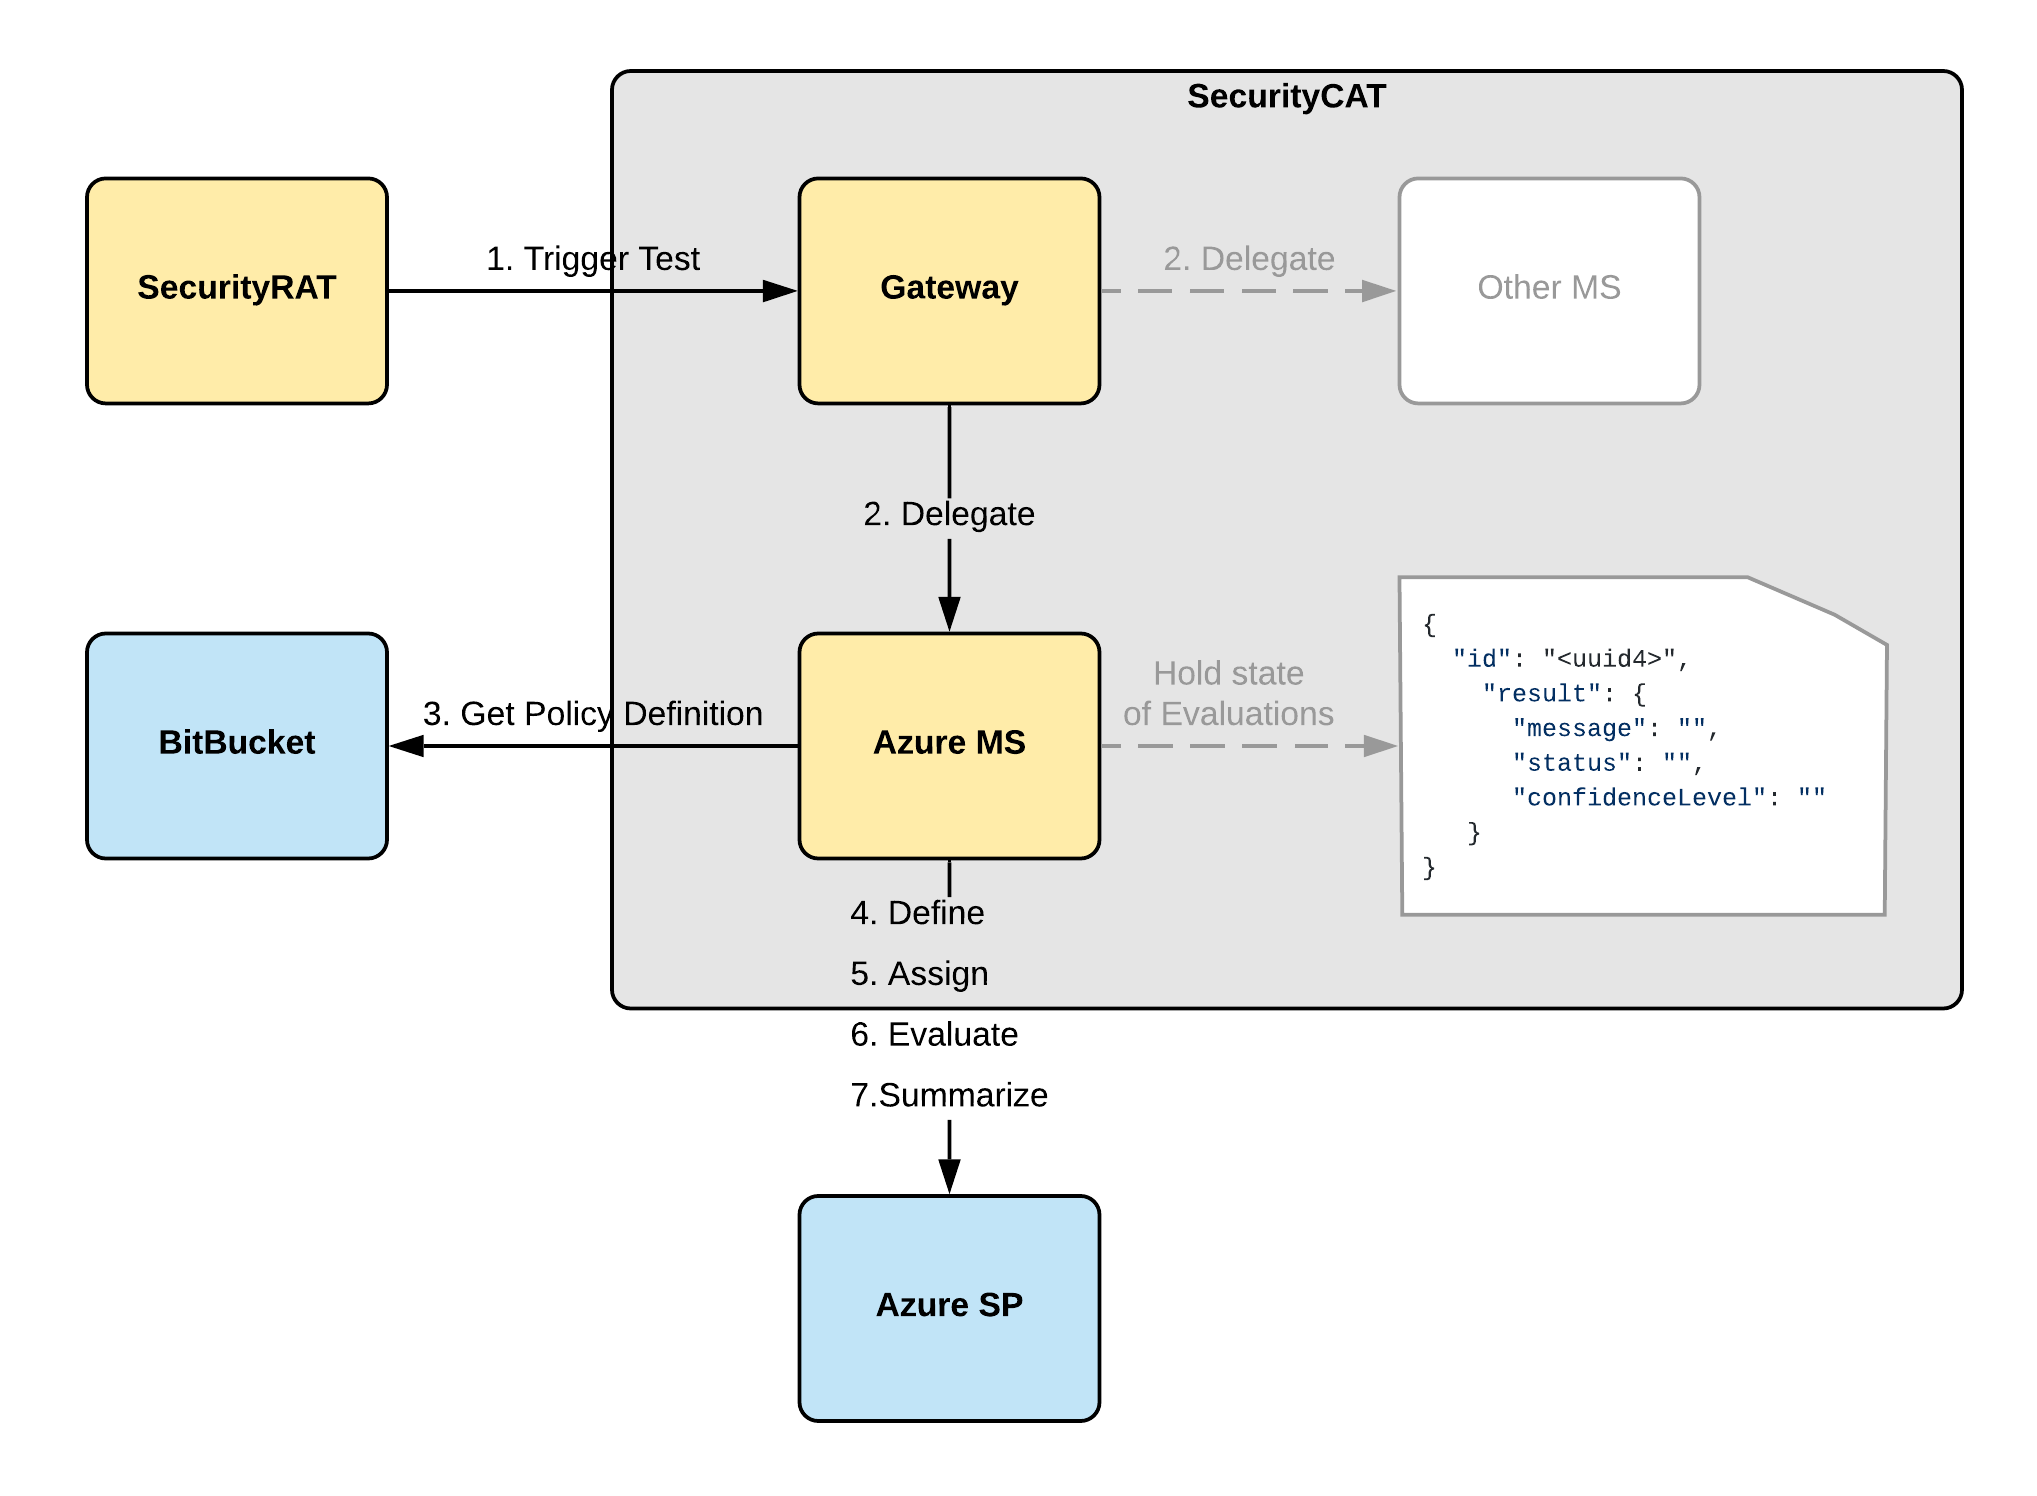
\includegraphics[width=15cm]{Azure_MS_flow.png}
\end{center}
\caption[SecurityRAT to Azure MS schema]{SecRAT to Azure MS schema}
%Source:
\end{figure}

Each Policy Evaluation is handled in a separate thread in the microservice. The policy definitions, assignments, and evaluations are done separately for each requirement.
The current state and final result of each evaluation are persisted in memory for the given evaluation-id. As described in \ref{architecture}, this is one of the critical sections of the architecture at the moment but can be easily replaced with a database in the progression from PoC to implementation. 

The definition, assignment, evaluation, and summarization flow is an essential part of the Azure microservice (Azure MS) since Azure requires a strict execution flow.
The main interaction flow between the microservice and Azure can be described as follows:

\newpage

\begin{figure}[ht!]
\begin{center}
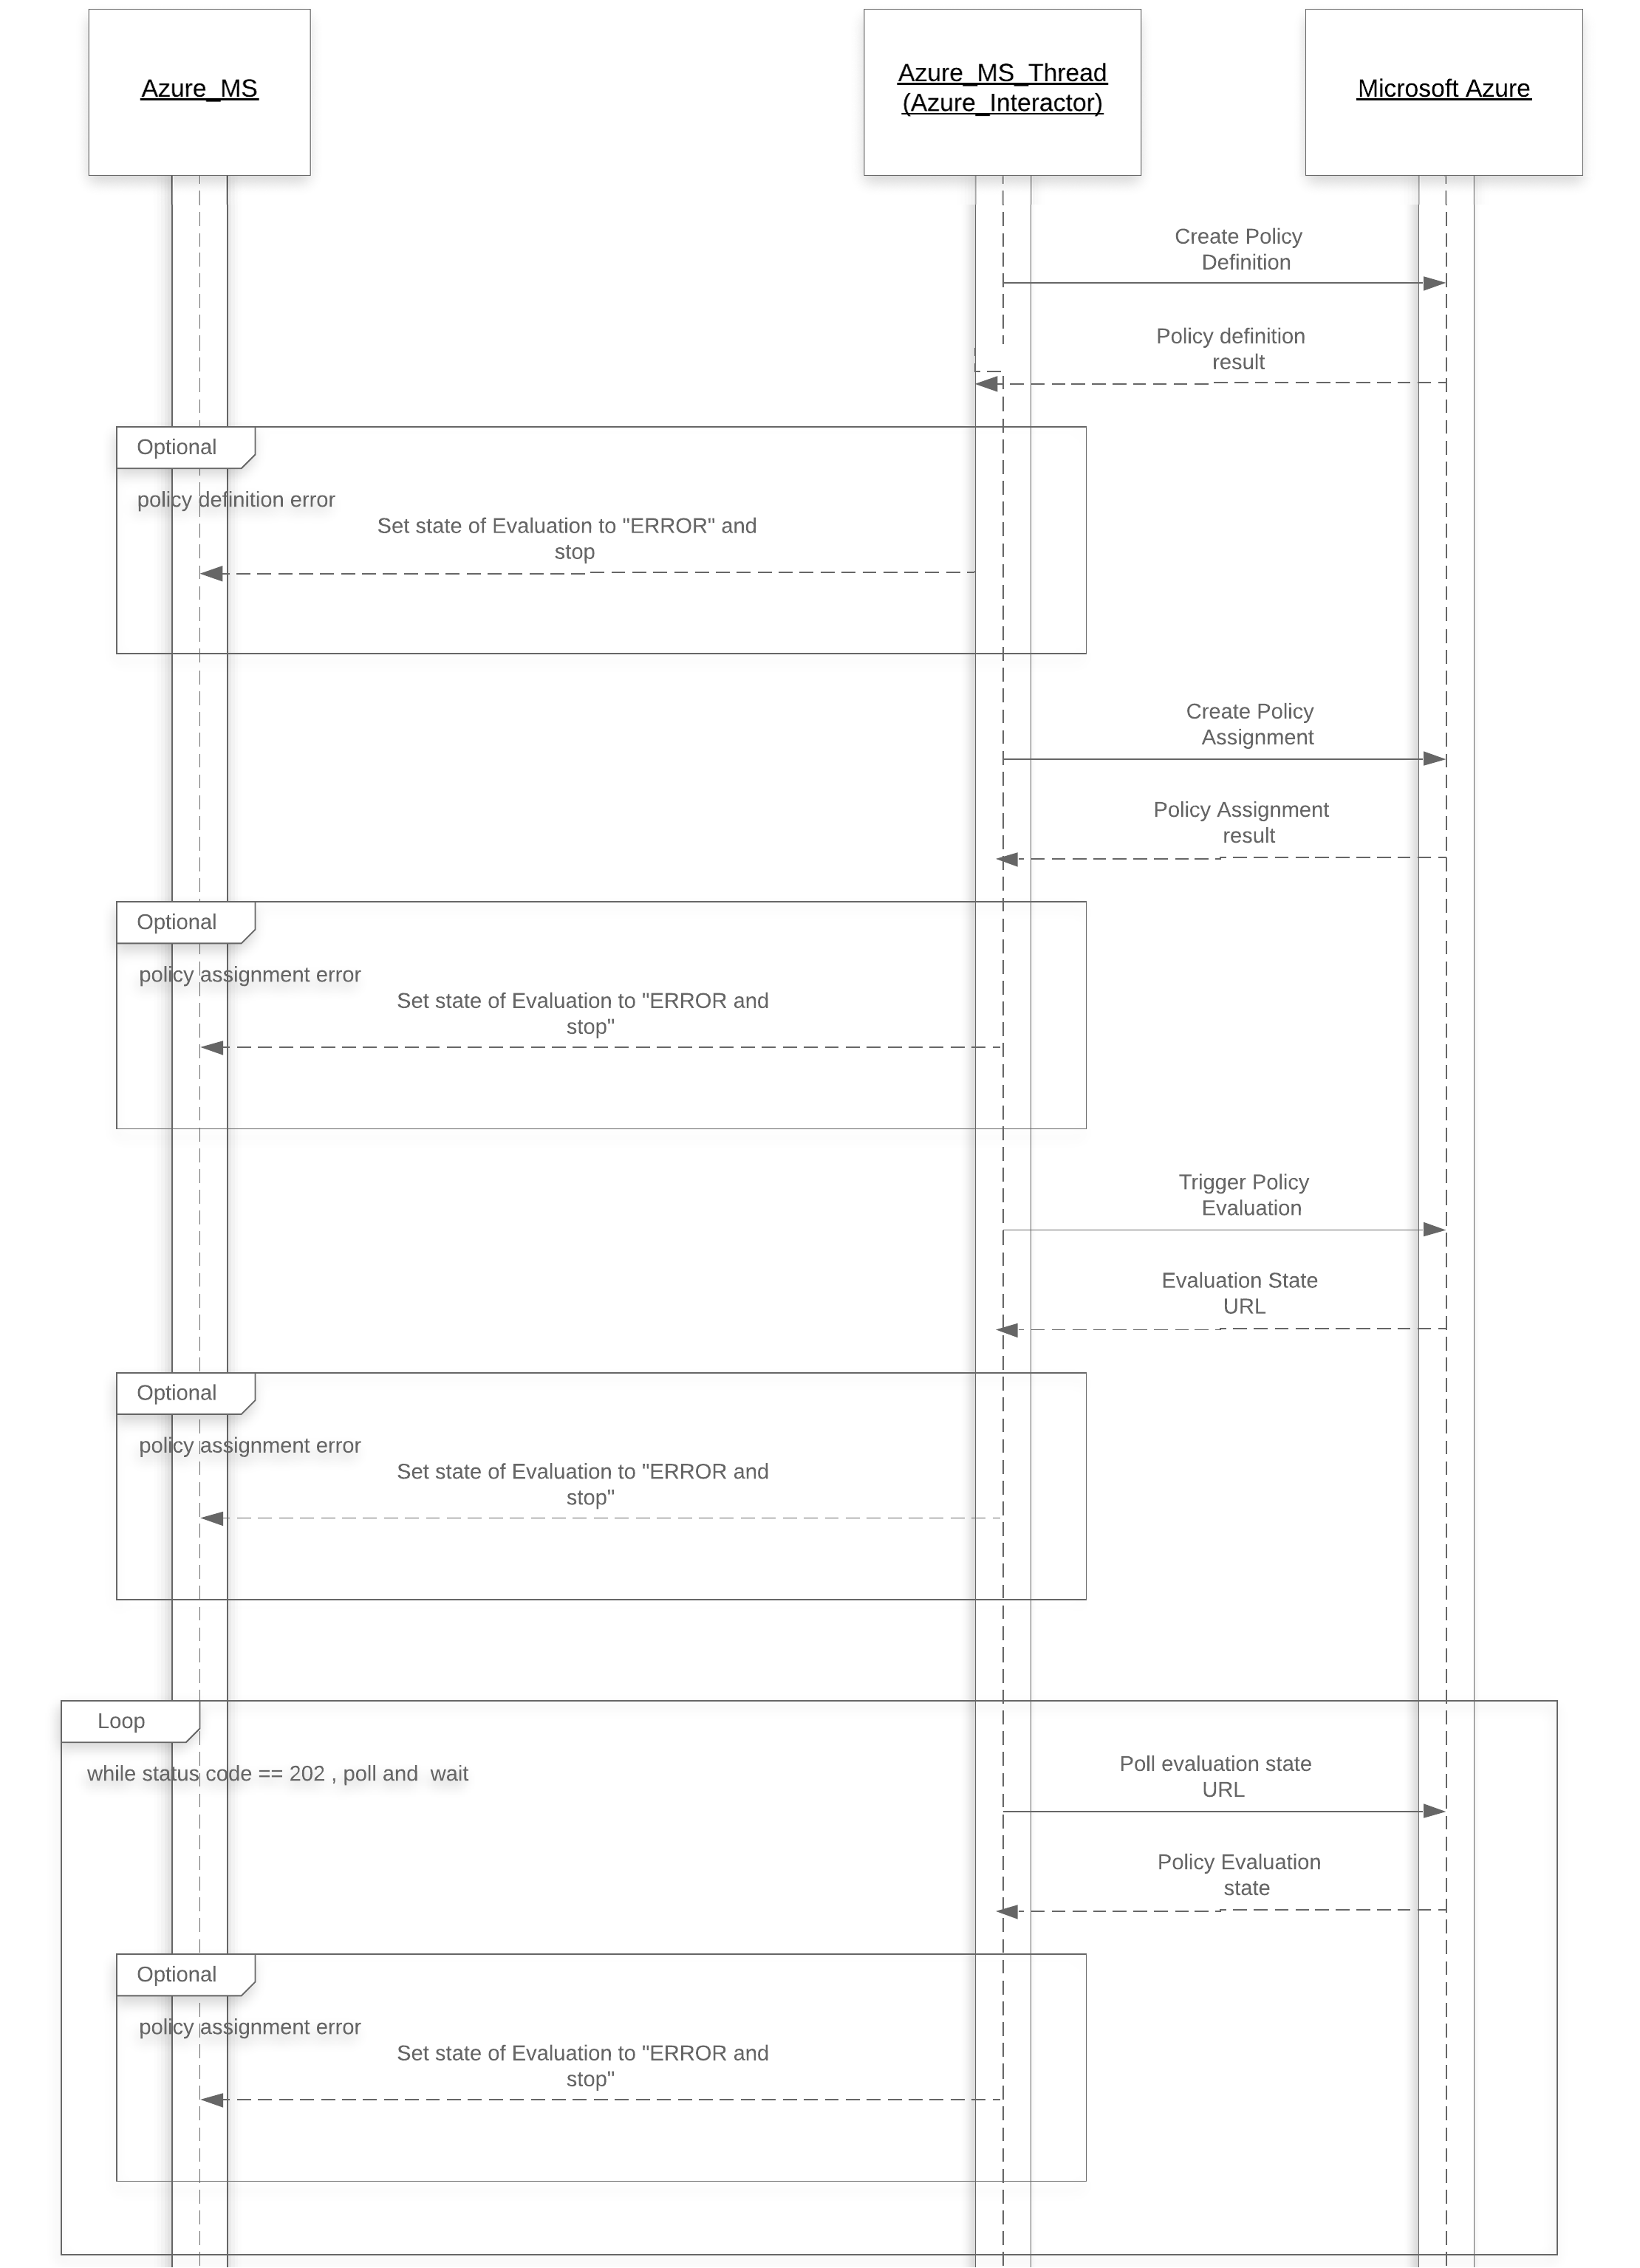
\includegraphics[height=20cm]{Azure_MS_Sequence_cropped.png}
\end{center}
\caption[Azure Policy MS sequence flow]{Azure Policy MS sequence flow. Full chart in Appendix \ref{azure_ms_sequence_chart}}
%Source:
\end{figure}

\vskip 1cm

The central part of the Azure microservice is the policy definitions. They define the expected behavior of a resource and can be tested against specific resources of the target system.

In order to get access to the Azure Policy system, a new application needs to be registered and authenticated using what is called a Service Principal. A service principal is bound to four pieces of information, a \boldsymbol{tenant\textunderscore id} of an Azure subscription, the \boldsymbol{client\textunderscore id} and \boldsymbol{token} (secret) of the registered application, and a \boldsymbol{resource} scope.

After the authentication process, policies can be uploaded, assigned, and triggered. The following example policy definition explains the structure and entities.

\vskip 1cm

\begin{lstlisting}[ backgroundcolor = \color{gainsboro}, 
                    xleftmargin = 2cm, 
                    framexleftmargin = 1em, 
                    language=JSON,
                    caption={Azure Policy Example},
                    captionpos=b]
{
"properties": {
    "displayName": "[MSA-0.0.1] - 
                        Single Contact in Subscription",
    "policyType": "BuiltIn",
    "mode": "Indexed",
    "description": "MSA-0.0.1 - Security contact must 
                                be set for Subscription",
    "metadata": {
      "category": "MSA"
    },
    "policyRule": {
      "if": {
        "field": "type",
        "equals": "Microsoft.Resources/Subscriptions"
      },
      "then": {
        "effect": "auditIfNotExists",
        "details": {
          "type": "Microsoft.Security/securityContacts"
        }
      }
    },
    "parameters": {}
  }
}
\end{lstlisting}

Each policy definition needs a \boldsymbol{displayName} that identifies the policy. The \boldsymbol{policyRule} section describes the targeted resources and expected behavior. In the example policy above, compliance is not achieved if security contact information is not given for Subscriptions.

Since the behavior of the check is defined through a standardized configuration file, the whole process of policy evaluation can be easily abstracted. 


\subsection{Amazon Web Services Config Rules}
\label{awsConfigRules}
Amazon Web Services (AWS) has a comparable system to test the compliance of infrastructure setup. The so-called, Config Rules are serverless Functions (Lambdas) that can be executed to test given resources for their compliance with the expected behavior.
Other than the simple policy definition configuration files on the Azure platform, the Config Rules are small programs written in one of the supported programming languages. This provides more powerful tooling to the user. However, it also increased the complexity of the creation process.

\newpage

Depending on the complexity of the Config Rule, Unit tests need to be added to ensure the correct working of the given script. AWS provides a list of useful config rules, like checking whether the volume encryption for computing resources is enabled. 

\begin{figure}[ht!]
\begin{center}
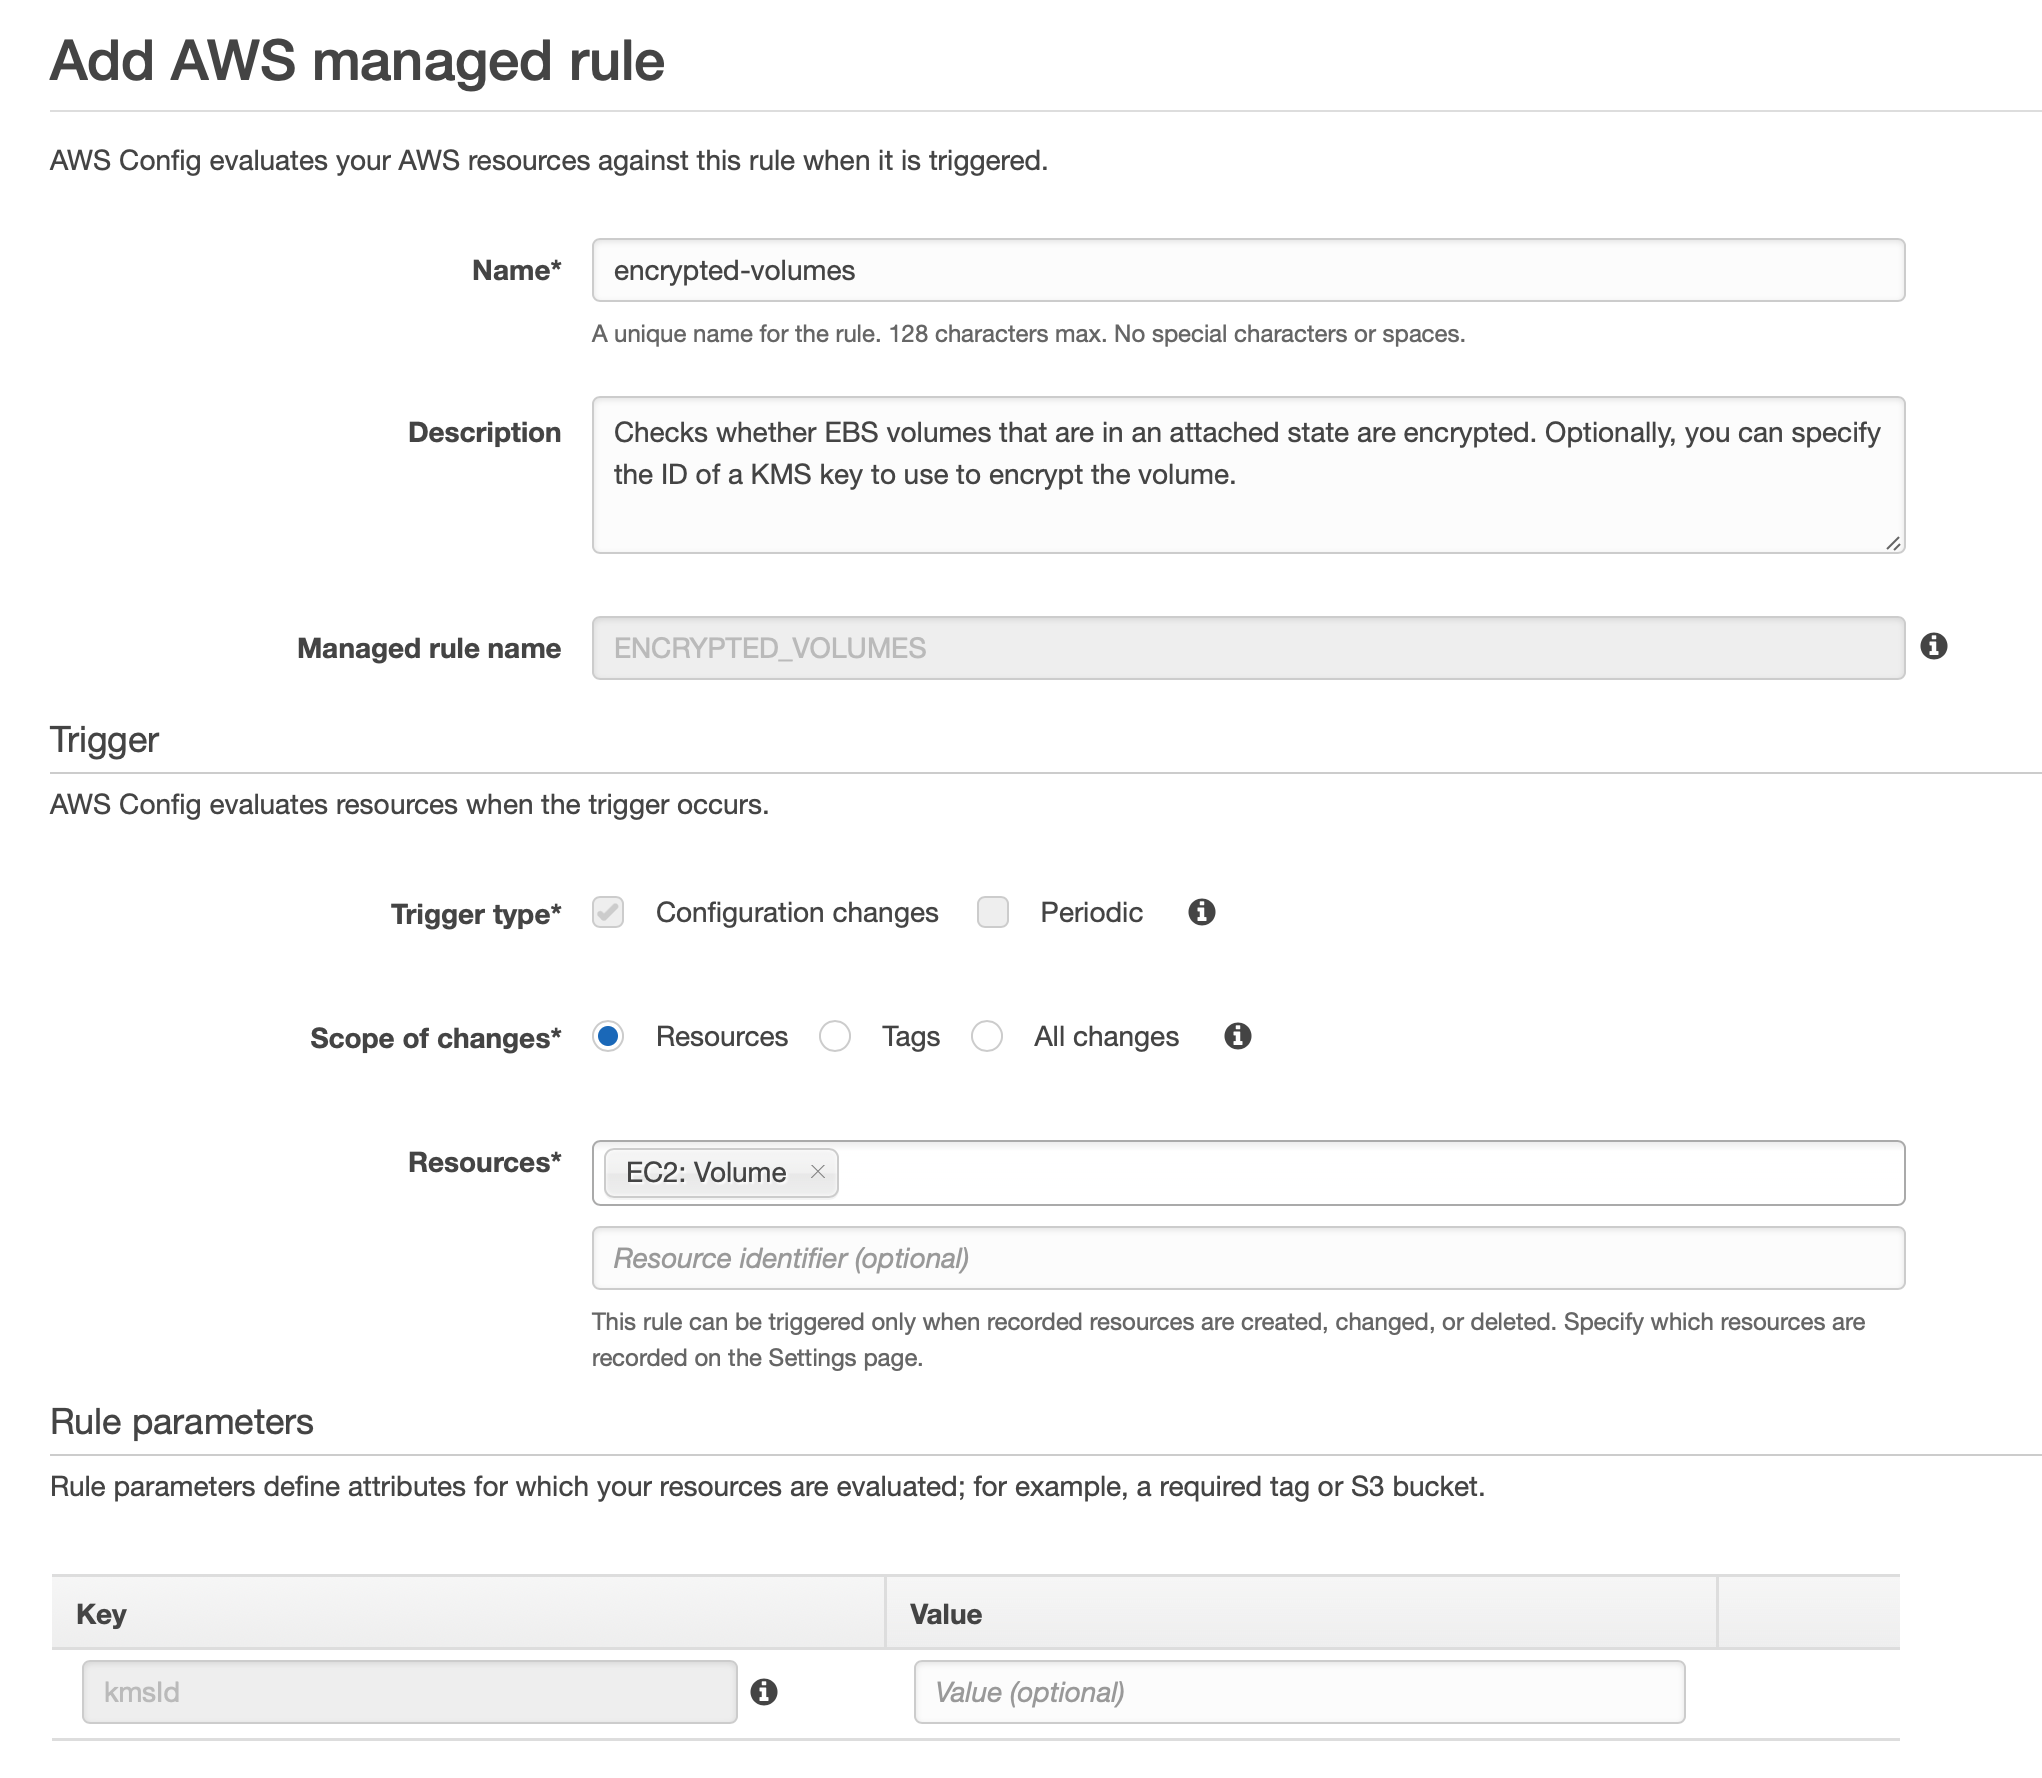
\includegraphics[width=15cm]{aws_config_rule_example.png}
\end{center}
\caption[EC2 Volume Encryption example Config Rule]{EC2 Volume Encryption example Config Rule}
%Source:
\end{figure}

In the AWS console, we can customize the provided config rules and define which resources should be affected and evaluated.
The management of the rules can be automated similarly, like the Azure Policies. A simple authentication flow, followed by describing, activating, and triggering the rule, can be created using the \boldsymbol{boto3} python library.

As part of this thesis, only one platform, Azure, has been covered and implemented.


\section{Automated Application Testing}
\subsection{Security Testing ZAP}
\label{zapTesting}
In contrast to infrastructure testing, applications have no strict underlying configuration that can be easily tested for misconfiguration using something like polices.
As briefly introduces in \ref{autoPentTesting}, the ZAP Proxy will serve as the automated security testing assessment tool for the PoC implementation.
The problems described in the conceptual chapter already introduced the existence of problems such as low confidence levels for problems and the vast amount of potential false negatives. When compared to automated infrastructure testing, we can not merely fully trust the results of the automated test but have to double-check manually.

\begin{figure}[ht!]
\begin{center}
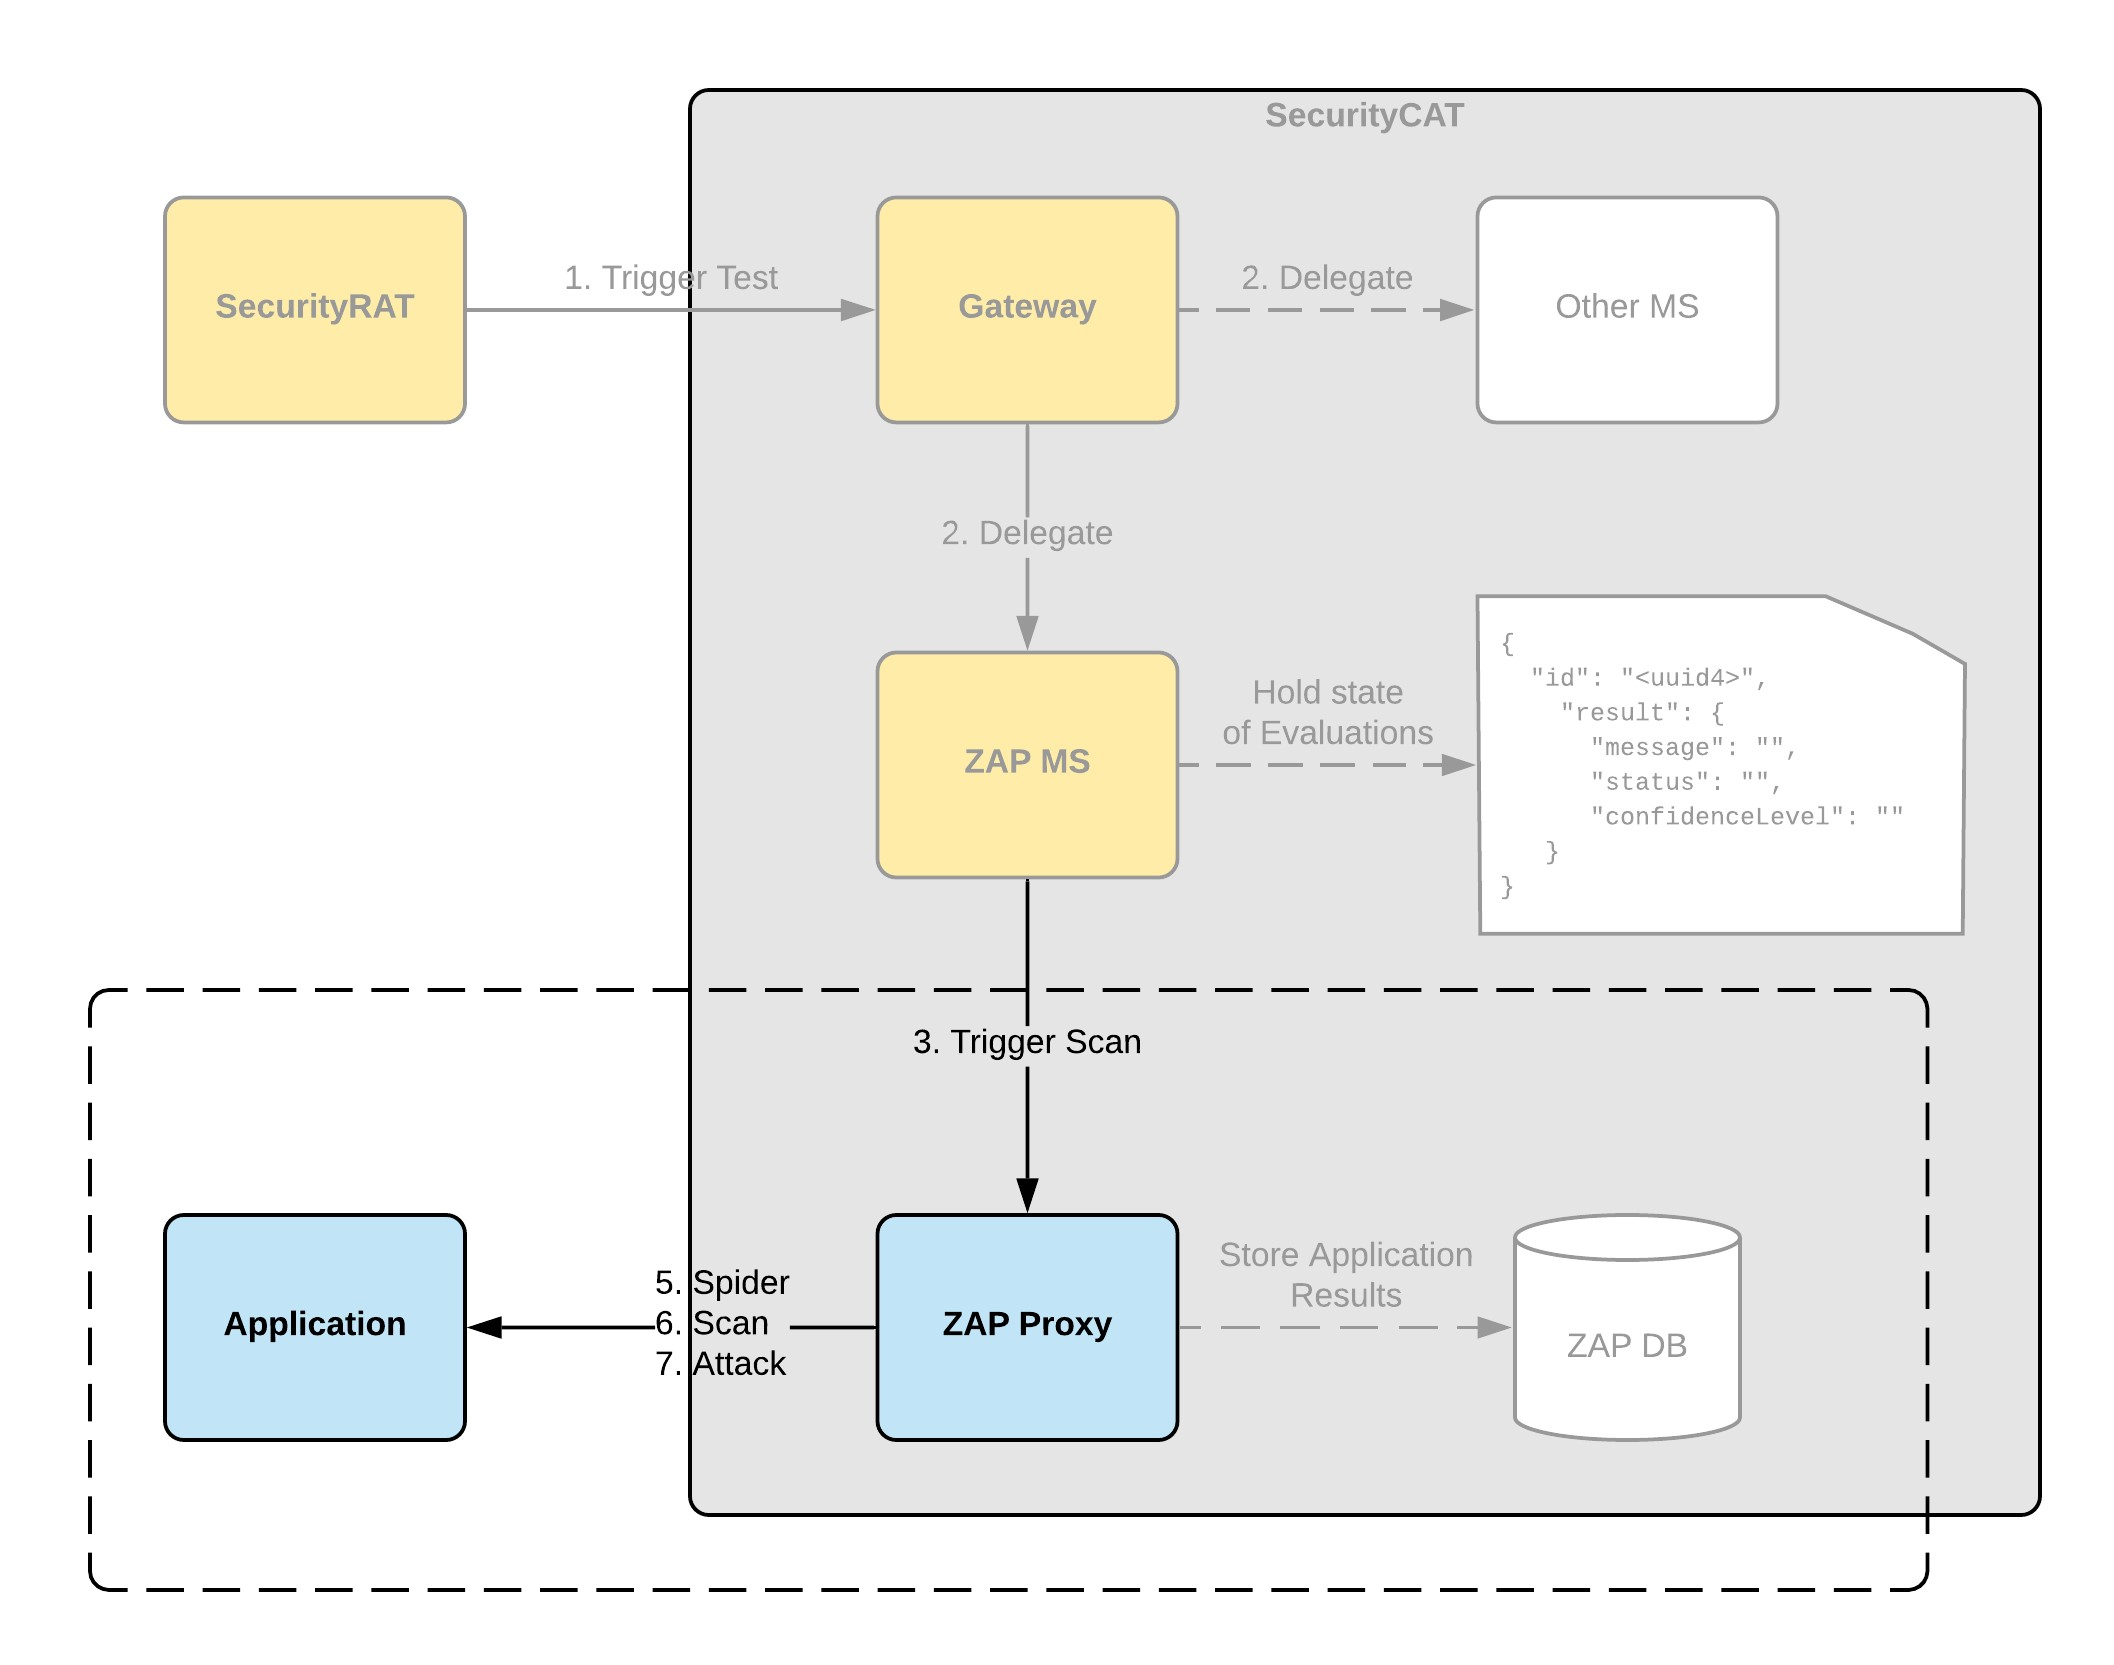
\includegraphics[width=15cm]{ZAP_MS_flow.jpg}
\end{center}
\caption[ZAP microservice flow with highlighted ZAP specific section]{ZAP microservice flow with highlighted ZAP specific section}
%Source:
\end{figure}

The schematic drawing shows the generally described format of the microservices and highlights the ZAP specific section of it. The microservice triggers the execution of a series of steps on a ZAP session. ZAP spiders, scans, and attacks the provided application and persists all found vulnerabilities and faulty configurations in its accompanying database. Once the full attack flow has been performed, the microservice gets the final report from the ZAP Proxy and provides the evaluation result for the querying of the gateway.

One problem with this approach is that ZAP only gives precise feedback. It can, for example, detect the presence of possibly security-critical information, exposed in the cookie header of a request. This information, however, has no direct mapping to one of the internal requirements that are listed in SecurityRAT.

The generated JSON report, therefore, has to get an additional mapping step, which helps categorize the found vulnerabilities and errors according to the internal requirements.
The structure of a found alert looks like this.

\vskip 1cm

\begin{lstlisting}[ backgroundcolor = \color{gainsboro}, 
                    xleftmargin = 2cm, 
                    framexleftmargin = 1em, 
                    language=JSON,
                    caption={ZAP Proxy \enquote{Header Not Set} Example Report},
                    captionpos=b]
{
   "alert":"X-Frame-Options Header Not Set",
   "riskcode":"2",
   "confidence":"2",
   "riskdesc":"Medium (Medium)",
   "desc":"<p>X-Frame-Options header is not included
          in the HTTP response to protect against
          'ClickJacking' attacks.<\/p>",
   "instances":[
      {
         "uri":"https://...",
         "method":"GET",
         "param":"X-Frame-Options"
      },
      .
      .
      .
   ],
   "count":"60",
   "solution":"<p>Most modern Web browsers...<\/p>",
   "reference":"<p>http://blogs.msdn.com/...<\/p>"
}
\end{lstlisting}

Each alert has some additional fields. Those fields, however, are not of value for now. The most critical pieces of information are the alert itself, its confidence, the riskdesc (severity), and the description. This information can be used to determine whether a requirement has failed or succeeded.

As mentioned above, since those results are dynamic and follow no strict model, they have to be manually checked for false positives. They can not be used as a final proof for a defined level of security.


\subsection{Custom Response Testing Script}
\label{customTestingScript} 
Standards like ASVS \citep{asvs4.0}, described in \ref{asvsStandard}, and an RFC of the HTTP/s protocol \citep{httpRFC} itself describe several security considerations when it comes to information transfer using HTTP/S.

Many of the given requirements specifically target the header values of an HTTP response. An example for this is the \enquote{ASVS\textunderscore 3.0.1\textunderscore 10.11} requirement which states the following:

\newpage

\begin{quote}
"Verify that HTTP Strict Transport Security headers are included on all requests and for all subdomains, such as Strict-Transport-Security: max-age=15724800; includeSubdomains"
\end{quote}

\vskip 1cm

Since HTTP headers are standardized, checking for their existence and value conformity can be automated. The response check microservice is aimed at not only testing the existence and value of headers for according to requirements but also provide an evaluation about the existence of non-compliant usage of weak encryption, encodings, and leaked session information. 

The following schema shows the response check microservice specific elements. The more specific "Requirement - Eval Function Mapping" entity is described in more detail in the next paragraph.

\begin{figure}[ht!]
\begin{center}
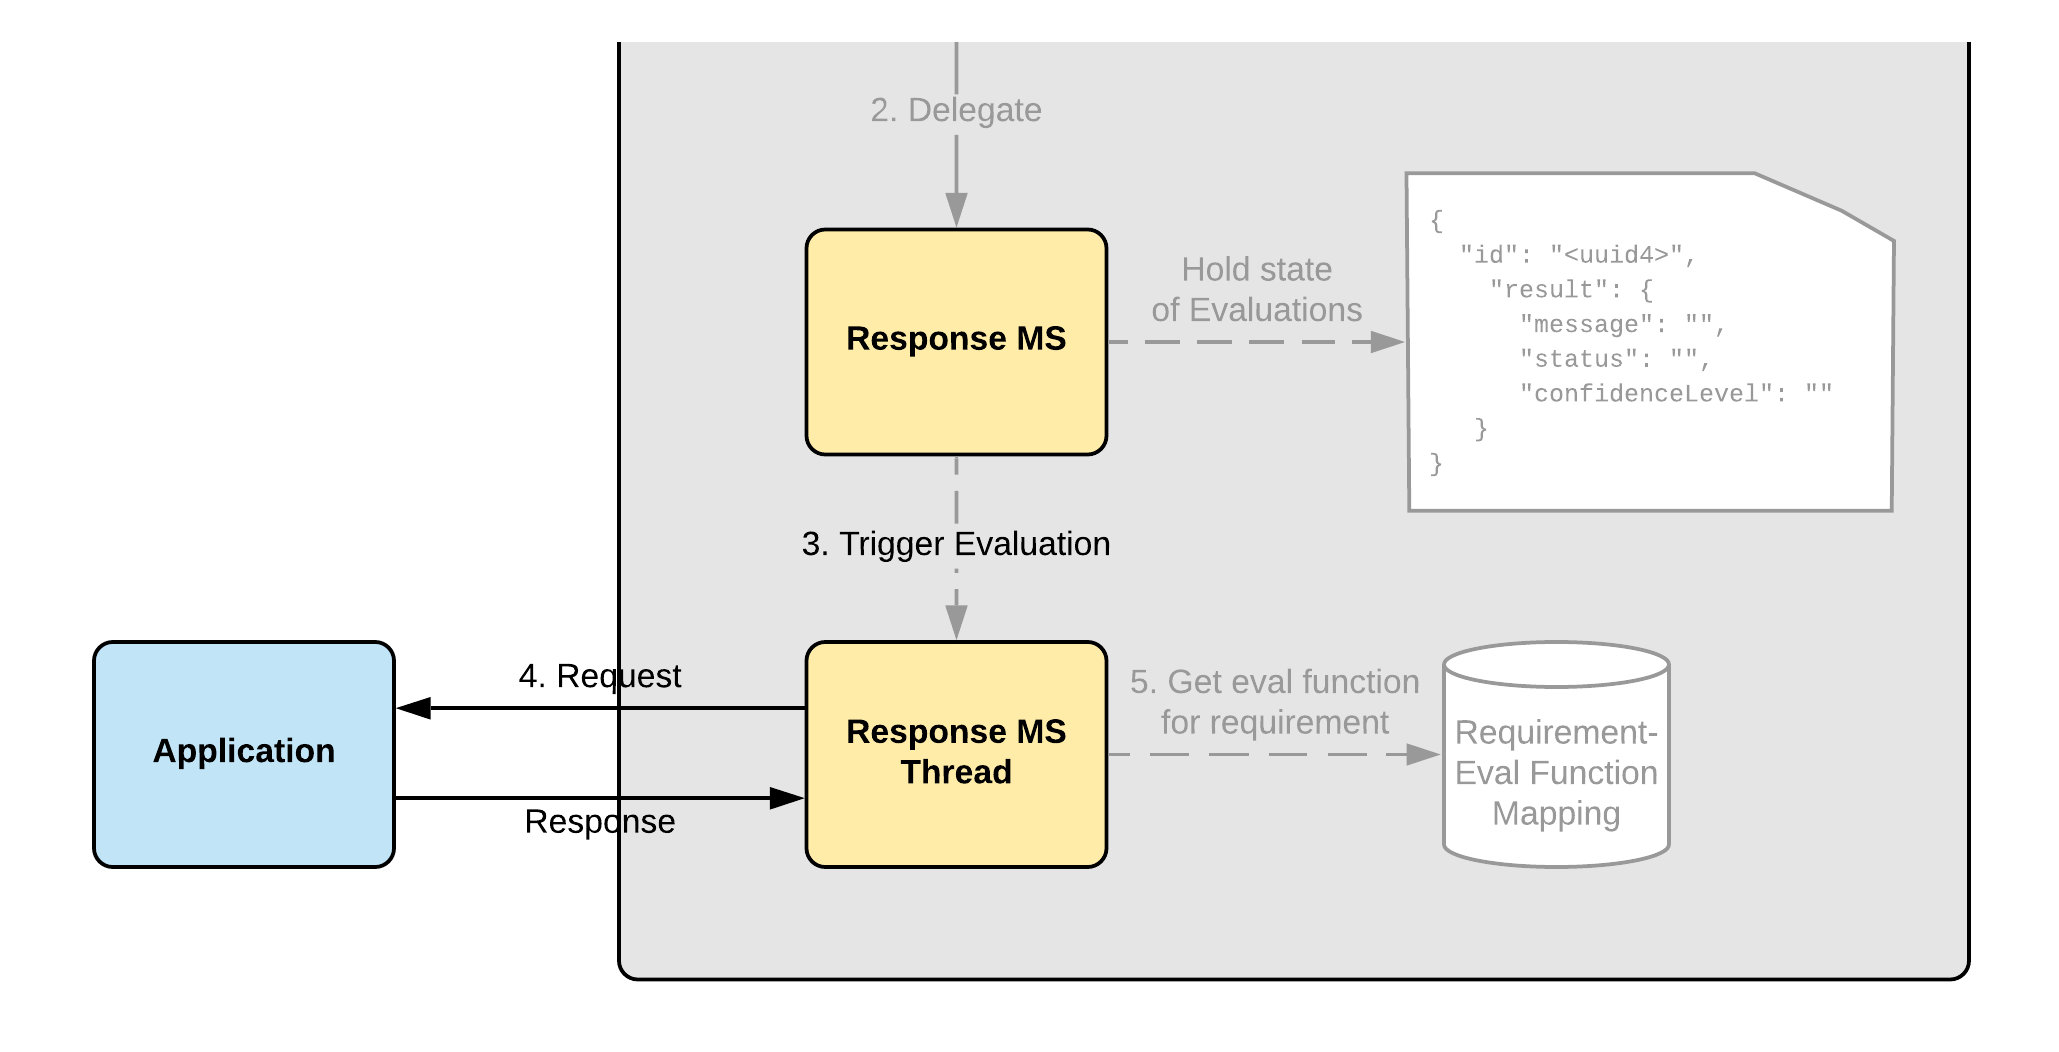
\includegraphics[width=17cm]{Response_Check_MS_flow.png}
\end{center}
\caption[Schematic flow of Response Check Microservice]{Schematic flow of Response Check Microservice}
%Source:
\end{figure}

\newpage

The approach taken for the response check microservice is focused on abstraction and dynamic extendability.
As displayed in the schema above, the basic structure of delegating the evaluation to a worker thread is consistent with all the other microservices.
One of the ways to achieve this abstraction is the introduction of a mapping entity. In a production environment, this can be a database; for this PoC, it is a simple in-memory dictionary. 
Each requirement is mapped to a function, which removes abstraction and provides specific instructions as soon as they become relevant for the evaluation. By using this structure, the implementation can be more general, which results in cleaner, more maintainable code. Requirements and functions can be added or removed at any stage.

The following code snippet displays an example mapping of three ASVS requirements to, so-called, lambda functions in Python.

\begin{lstlisting}[ backgroundcolor = \color{gainsboro}, 
                    xleftmargin = 2cm, 
                    framexleftmargin = 1em, 
                    language=Python,
                    caption={ASVS Requirements to Function mapping},
                    captionpos=b]
__requirement_func_mapping = {
  "ASVS_3.0.1_10.10": lambda headers: 
      __check_headers_contains_elem(
        headers, "Public-Key-Pins"
      ),
  "ASVS_3.0.1_10.11": lambda headers: 
      __check_headers_contains_elem(
        headers, "Strict-Transport-Security"
      ),
  "ASVS_3.0.1_10.12": lambda headers: 
      __check_headers_contains_elem(
        headers, "Strict-Transport-Security", "preload"
      ),
}
\end{lstlisting}

Over time, this microservice should be enriched with a more sophisticated analysis of the HTTP response of the client application. Possible checks include the usage of insecure encodings, exposed session information, guessable session ids, and other, previously mentioned, security considerations.
An important aspect also is the mapping of functionality to the internal requirements maintained by the team. Since those requirements are more general than ASVS, the second step of mapping might need to be introduced upon further experimentation.


\section{Extendability}
\label{extendability}
Considering the architecture described in \ref{architecture}, adding new microservices and extending the system is a streamlined process. As more requirements can be tested, additional microservices can be implemented to evaluate them. Each microservice needs to implement the informal interface in order to keep the communication to the gateway consistent.

Since Python has no concrete concept of interfaces, the approach used here is a very informal one. Documentation and examples should provide a guideline on how new microservices have to be implemented. Once the PoC surpasses the stage feasibility checking, a formal interface based on the used guidelines shall be implemented with the Python-specific tooling.

Each microservice exposes a GET and a POST REST endpoint. A new evaluation is triggered by posting the definition to the POST endpoint. In the example of the Azure policy microservice, this definition is the \boldsymbol{PolicyEvalDefinition} shown in the figure above. This POST call starts a new evaluation and returns the associated \boldsymbol{eval\textunderscore id} to the gateway.
By using the GET endpoint with the given \boldsymbol{test\textunderscore id}, the current state of evaluation and the result, once the evaluation has finished, can be retrieved.

\begin{figure}[ht!]
\begin{center}
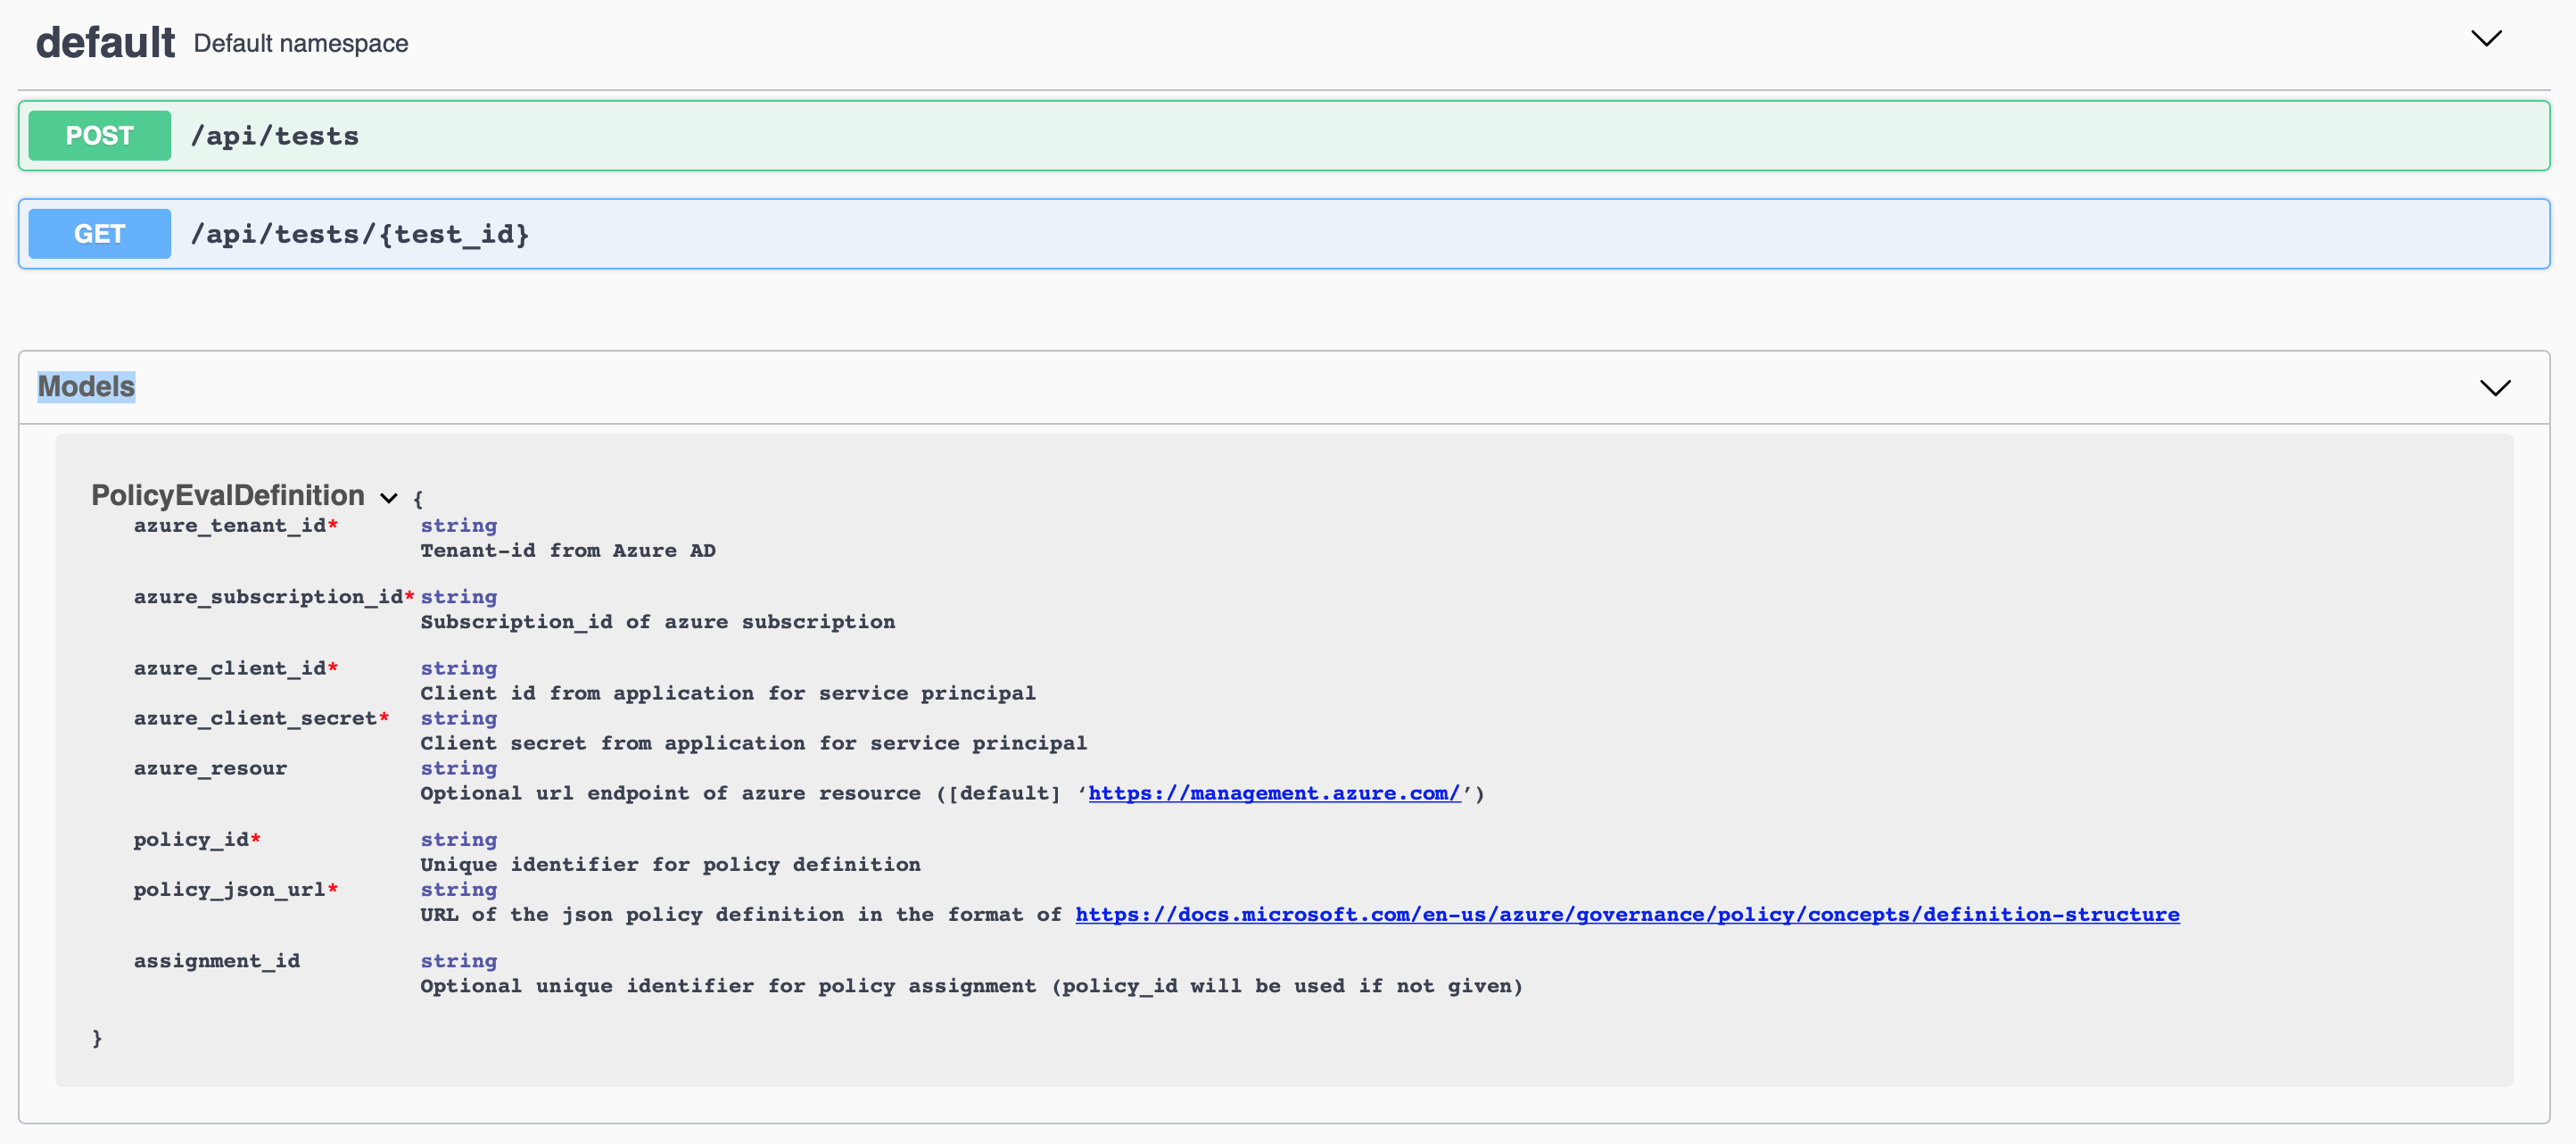
\includegraphics[width=17cm]{swagger_api_azure.png}
\end{center}
\caption[Swagger API documentation of the Azure microservice]{Swagger API documentation of the Azure microservice}
%Source:
\end{figure}
\addchapheadtotoc
\chapter{Evaluation}
\label{evaluation}

This chapter gives an evaluation of feasibility for each of the implemented microservices and points out pitfalls and drawbacks as well as advantages. A final outlook lists elements of concern that need to be covered in future efforts to leverage the full potential of the automation system.

\section{Azure Microservice}
The policy evaluation and compliance service of Azure already provide all the functionality required to test the system resources. Running additional tests on the \enquote{correctness} of their evaluations would be a waste of time. A second advantage of delegating the evaluation to a thoroughly tested cloud service is the high confidence we can assign for \enquote{Passed} or \enquote{Failed} tests. 
Since the implementation of this PoC has no underlying SLAs (Service Level Agreements), even the run-time of the Azure microservice can be neglected.

However, uncovering potential lengthy running evaluations and providing an indication of possible wait times when running the automated testing pipeline can be of great value for the evaluation of the feasibility of using the Azure microservice in production. Therefore, some runtime tests have been made by executing the same evaluation on the same system ten times. The tests were conducted on the currently used Azure Subscription of the security team at ETAS SEC/ECT-Fe with 176 to be evaluated policies active in the compliance scope. According to \citep{stackoverflowTrigger}, only executing a single compliance check of a given policy is possible. This, however, has to be investigated further outside the scope of this thesis. 

\begin{table}[htb]
\begin{tabular}{|l|l|l|l|l|l|l|l|}
\hline
\textbf{Run} & \textbf{Init} & \textbf{Def} & \textbf{Assign} & \textbf{Trigger} & \textbf{Poll} & \textbf{Result} & \textbf{Total} \\ \hline
1            & 1.7217        & 2.273        & 0.4247          & 0.8354           & 495.3885      & 0.2503          & 500.8941       \\ \hline
2            & 1.7406        & 2.2096       & 0.4401          & 0.8000           & 497.7047      & 0.2558          & 503.1510       \\ \hline
3            & 1.6200        & 2.1100       & 0.4400          & 0.4597           & 432.9334      & 0.2495          & 437.8129       \\ \hline
4            & 1.7029        & 2.1439       & 0.4402          & 0.8182           & 744.4237      & 0.2742          & 749.8034       \\ \hline
5            & 1.6499        & 2.0804       & 0.4397          & 0.4901           & 557.6947      & 0.5737          & 562.9288       \\ \hline
6            & 1.7419        & 2.5185       & 0.4397          & 0.5602           & 558.2836      & 0.2810          & 563.8251       \\ \hline
7            & 1.8458        & 2.1392       & 0.4595          & 0.4974           & 557.0948      & 0.2902          & 562.3272       \\ \hline
8            & 1.7432        & 2.0071       & 0.4360          & 0.8539           & 620.9929      & 0.5996          & 626.6329       \\ \hline
9            & 1.7433        & 2.0500       & 0.4666          & 0.8832           & 742.9784      & 0.2385          & 748.3602       \\ \hline
10           & 1.6376        & 2.3524       & 0.5124          & 0.8138           & 731.1293      & 0.2974          & 736.7433       \\ \hline
\end{tabular}
\caption{Execution time taken (in seconds) for the phases of the Azure Microservice}
\end{table}

\newpage

The rows of the table above are identified in the following way:
\begin{itemize}
    \item $\boldsymbol{Run}$ - id of the run
    \item $\boldsymbol{Init}$ - time taken to initialize the thread and authenticate with Azure
    \item $\boldsymbol{Def}$ - time taken to create the policy definition
    \item $\boldsymbol{Assign}$ - time taken to create the policy assignment
    \item $\boldsymbol{Trigger}$ - time taken to trigger the evaluation of assigned policy
    \item $\boldsymbol{Poll}$ - time taken for the evaluation (result polled every 10s)
    \item $\boldsymbol{Result}$ - time taken to retrieve the result from azure
    \item $\boldsymbol{Total}$ - summed up time taken for the full evaluation
\end{itemize}

A glance at the numbers in the table provides some necessary information about the run time of each phase of the policy evaluation. To better understand the run-time impact of each phase, the mean and standard deviation for each phase are calculated and plotted on a logarithmic scale chart to avoid the squashing of the low values compared to the \boldsymbol{Poll} column.

\begin{figure}[ht!]
\begin{center}
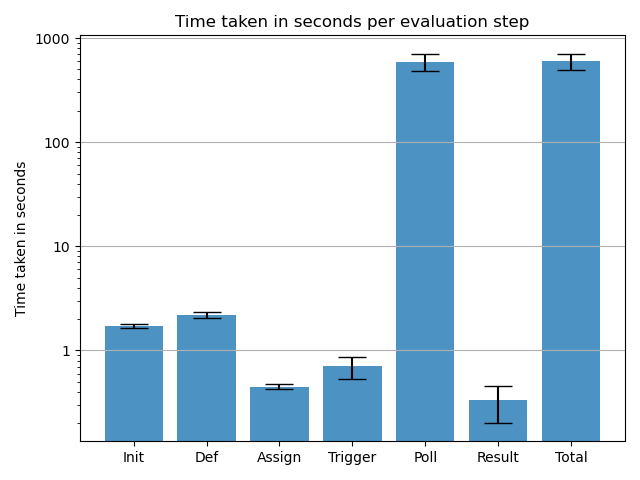
\includegraphics[width=15cm]{azure_evaluation_time.png}
\end{center}
\caption[Mean evaluation time of each phase with standard deviation plotted as bar chart]{Mean evaluation time of each phase with standard deviation plotted as bar chart}
%Source:
\end{figure}

The chart shows the mean run-time over 10 test runs for each phase as a separate bar. The black ranges indicated at the top of the bar charts display the standard deviation.
The Y-Axis indicates that all phases other than the polling - which includes the resource evaluation on Azure - can be ignored for this PoC. As mentioned before, the evaluation, as of now, trigger the whole suite of assigned policies instead of only one. Polling resides somewhere between 433 and 744 seconds. However, time not essential since executing the automated tests does not block SecurityRAT while the evaluation is going on.
In addition to that, explicitly triggering the evaluation of a single policy will decrease the run-time of the evaluation significantly. The function-based Config Rules in AWS \ref{awsConfigRules} have the advantage of being separately triggerable by nature, which results in a more suitable run-time.


\section{Response Check Microservice}
\label{refResponseCheckMS}
In contrast to the Azure microservice, run-time is not a significant concern of the Response Check microservice. As mentioned before, the company internal requirements are held very general, at least compared to, for example, the ASVS. This poses the difficulty of having a particular set of tests to be done in order to \enquote{Pass} a given requirement.

A possible solution for this has been described in \ref{customTestingScript}. By using a pseudo-database to map each requirement to a function that can hold any combination of tests according to the requirement, the problem of not having a clear definition of what has to be tested can be solved. In this case, an expert has to write the tests once. After that, they can be re-used for all other executions.

The implementation of this PoC only provides three examples based on the ASVS definition already used in \citep{secCat2020}, in a more abstracted and extendable manner. However, since the goal of this microservice is to test the feasibility of this approach and considering the vast diversity of requirement sets used in security compliance testing, providing an adaptable system is the main focus.

Further tests will show whether moving from a single, multi-requirement test to multiple, single-requirement tests pipeline will only increase the load of tasks, or deliver the expected advantages of further decoupling each requirement. This should avoid elongated executions or loss of state due to the blocking of short running evaluations or failing of evaluations. This refactor, of course, increases the work done by the gateway, which only should proxy the required evaluations to the microservices. For the scope of the PoC implemented in this thesis, this trade-off has been preferred.


\section{ZAP Microservice}
In order to test the ZAP microservice, run-time and result have been briefly analyzed to evaluate the feasibility of using an automated penetration testing tool as part of SecurityCAT.
The following tests have been done on the OWASP Juice Shop using the default settings for the ZAP Proxy. The default spider, Ajax spider, and active scanning have been used.
A crucial piece of information is that the \enquote{Runs} build on top of each other, meaning that the information found in the first run is used to conduct a more in-depth search in the second execution. This deepening of search space is prominent when looking at the \enquote{Runtime} row of the table. It indicates a possible exponential increase in run-time.

\newpage

\begin{table}[]
\begin{tabular}{|l|l|l|l|l|}
\hline
\textbf{Run}            & \textbf{1} & \textbf{2} & \textbf{3} & \textbf{4} \\ \hline
\textbf{Runtime (s)}    & 173.0392   & 314.6481   & 1054.3518  & 5688.1767  \\ \hline
\textbf{Alerts}         & 366        & 2799       & 11414      & 57176      \\ \hline
\textbf{Low}            & 137        & 1538       & 7587       & 41515      \\ \hline
\textbf{Medium}         & 129        & 936        & 3269       & 14877      \\ \hline
\textbf{High}           & 0          & 2          & 2          & 3          \\ \hline
\textbf{Grouped Alerts} & 10         & 13         & 13         & 13         \\ \hline
\textbf{Low}            & 5          & 6          & 6          & 6          \\ \hline
\textbf{Medium}         & 2          & 3          & 3          & 3          \\ \hline
\textbf{High}           & 0          & 1          & 1          & 1          \\ \hline
\end{tabular}
\caption{ZAP MS evaluation statistics}
\end{table}

With only one run, however, we were not able to find the \enquote{High} risk alert, which in this case, is a SQL Injection to log in as administrator.
This surfaces the problem that several executions might need to be executed in order to get any suitable result. Judging by the \enquote{explosion} of run-time over the four runs, this, however, is not feasible for the automation approach taken as part of this thesis.

Since the run-time escalation is a severe problem, for the scope of this thesis, no mapping has been implemented for the ZAP microservice yet. However, the mapping system introduced in \ref{refResponseCheckMS} provides a good baseline for further tests for the ZAP microservice.

As mentioned in \ref{drawbackAutomated}, automated penetration and vulnerability tests introduce a lot of false positives and are lacking the \enquote{expertise} of finding actual vulnerabilities.
Most results of ZAP only have a \enquote{medium} or \enquote{low} confidence level, which does not eliminate the need for manual checking and, therefore, reduce the benefit of such automated tests. 

The RAII (Resource allocation is initialization) principle, used in the creation process of new evaluations, works well for unauthorized API calls. A wrong API key instantly errors the evaluation and returns this status in the evaluation creation step. Therefore no evaluation session is started if the requester is not authorized.

In order to test the feasibility of using this automated penetration testing approach as part of the SecurityCAT setup, a demo application has to provide for tests in combination with the implemented internal requirements. Alternatively, additional tests with one of the famous test applications, like the OWASP Juice-Shop, can be conducted after an expert has analyzed it, and met requirements have been identified.


\section{Outlook}
The sections above already describe some of the drawbacks and potential points of failure of the implemented microservices. In addition to those, the full system has not been combined for testing. Each microservice was tested separately in combination with the gateway. Instead of SecurityRAT, the SwaggerAPI of the gateway was used to conduct the tests.
One of the next steps, therefore, is to combine SecurityCAT with SecurityRAT and run end-to-end tests for the whole pipeline.

One \enquote{drawback} of a microservice system are the many decoupled components. Starting and setting up the environment can be time-consuming and error-prone, repetitive work. By using containers and a docker-compose setup in the future, the whole system can be torn down and re-build automatically in no time.  

Additional thoughts have to be put into how to assign the requirement a more defined \enquote{YES} or \enquote{NO} according to the evaluation result. This concern is especially crucial for the ZAP and Response Check microservices. As described before, they carry a high chance of resulting low confidence results that could introduce more problems which, in the long run, would result in more work.
\chapter{Summary and Conclusion}
This thesis tries to provide an approach to automate parts of the security and compliance check process for software systems.
The proof of concept implementation of the security compliance automation tool (SecurityCAT) aims to simplify this process by providing a decoupled set of microservices capable of automatically evaluating the compliance state of requirements.

The requirement management tool of choice, SecurityRAT, enables the use of SecurityCAT through an exposed API. The integrated polling mechanism defines the architecture described in \ref{architecture}. As a single source of truth, only results pulled into SecurityRAT define requirements as evaluated.

In theory, automating compliance checks is an important and even essential idea. However, as described in \ref{evaluation}, it comes with many drawbacks and uncertainties since the complexity of the task requires more sophisticated approaches. When leveraging the capabilities of cloud providers like Microsoft Azure or AWS, handling the complexity is delegated to their services.
The promising results of the Azure microservice elevate from the above-given statement.

For less complex tasks like checking the provided headers of an HTTP response, simple scripting can be used to get passable results. This manual scripting and configuration for the given requirement set, however, still requires a domain expert in the loop. In larger corporations, security experts could create a central database of requirement to evaluation functions, which would shift the need for expertise to one central entity.

The nearly infinite attack space of an application is what makes automated security vulnerability testing difficult. As described in \ref{drawbackAutomated}, merely launching a suite of attacks against an application seldomly leads to high confidence findings.
In addition to the uncertainty, the high run-time of scans might lead to problems with simultaneous evaluations running.

Each microservice comes with a suite of drawbacks that have to be evaluated in more detail. The Azure and Response Check microservices serve as a solid start for further investigation. The ZAP microservice, in contrast, might require a different approach to be more useful in the given environment.

In conclusion, the need for automated security testing will support the further development of automation tooling. SecurityCAT is only one of many approaches, discussed in this thesis and referenced in \ref{relatedWork}.
Further testing and improvements on the tool will show if it can be safely integrated into the current testing workflow and provide benefits to the users of security management tools like SecurityRAT.

% Appendices
\appendix

%%%%%%%%%% DON'T DELETE THIS, REVERTS NUMBERING BACK %%%%%%%%%%%%%
\makeatletter
\renewcommand{\@makechapterhead}[1]{\vspace *{-10\p@ }{\parindent \z@ 
\raggedright \normalfont \ifnum \c@secnumdepth >\m@ne \Huge \bfseries 
\@chapapp \space \thechapter \vskip 10\p@ \fi #1\par \nobreak \vskip 30\p@ }}
\makeatother
%%%%%%%%%% DON'T DELETE THIS, REVERTS NUMBERING BACK %%%%%%%%%%%%%

\chapter{Azure Microservice Sequence Chart}
\label{azure_ms_sequence_chart}
\vspace*{-0.3in}
\begin{figure}[hb!]
\begin{center}
\makebox[\textwidth][c]{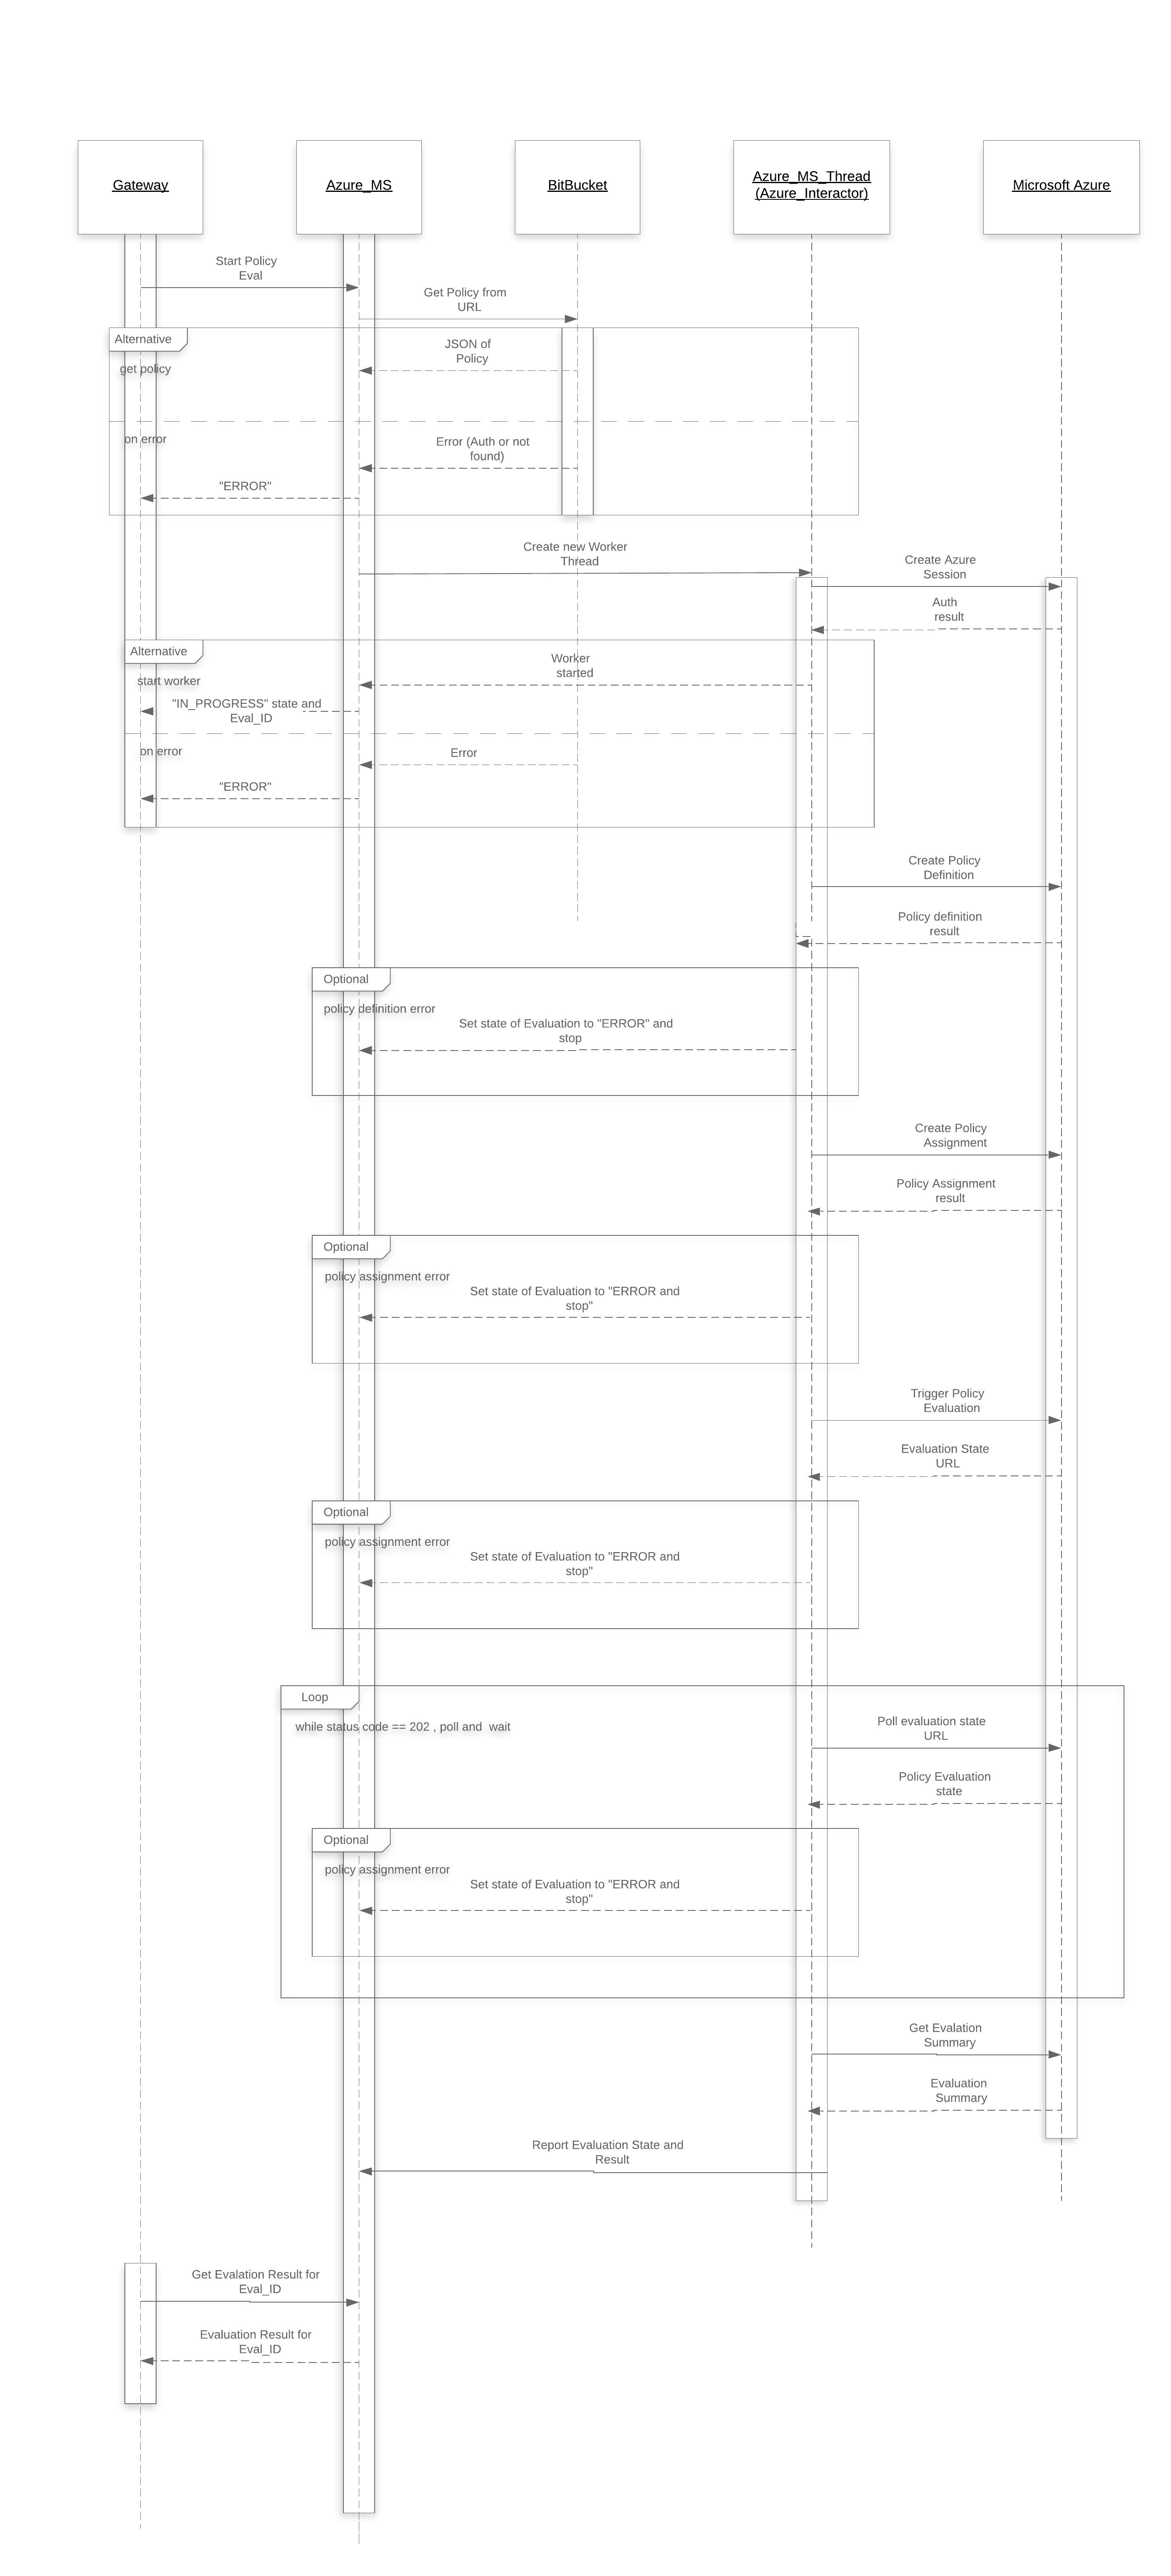
\includegraphics[height=16cm]{Azure_MS_Sequence.png}}
\end{center}
\caption[Sequence chart of Azure MS Policy creation flow]{Sequence chart of Azure MS Policy creation flow}
\end{figure}

% Bibliography
\begingroup
    \setlength\bibitemsep{10pt}
    \linespread{1}\selectfont
    \printbibliography[title=References]
\endgroup
\addcontentsline{toc}{part}{References}

\end{document}
